%%%%%%%%%%%%%%%%%%%%%%%%%%%%%%%%%%%%%%%%%%%%%%%%%%%%%%%%%%%%%%%%%%%%%%%%%%%%
%% Author template for Marketing Science (mksc)
%% Mirko Janc, Ph.D., INFORMS, mirko.janc@informs.org
%% ver. 0.95, December 2010
%%%%%%%%%%%%%%%%%%%%%%%%%%%%%%%%%%%%%%%%%%%%%%%%%%%%%%%%%%%%%%%%%%%%%%%%%%%%
\documentclass{informs_mod} % current default for manuscript submission
%\documentclass[mksc,nonblindrev]{informs3}

%%\OneAndAHalfSpacedXI % current default line spacing
\OneAndAHalfSpacedXII
%%\DoubleSpacedXII
%%\DoubleSpacedXI

% If hyperref is used, dvi-to-ps driver of choice must be declared as
%   an additional option to the \documentclass. For example
%\documentclass[dvips,mksc]{informs3}      % if dvips is used
%\documentclass[dvipsone,mksc]{informs3}   % if dvipsone is used, etc.

% Private macros here (check that there is no clash with the style)
% Cross reference package
\usepackage{cleveref,morefloats,rotating,graphicx,multirow,tabularx}
\usepackage{amsmath, amsthm, amssymb} % Math packages
\usepackage[caption=false]{subfig}
\renewcommand\thesubfigure{(\alph{subfigure})}

%% setup subfigure captioning
\captionsetup[subfigure]{subrefformat=simple,labelformat=simple}

% Natbib setup for author-year style
\usepackage{natbib}
 \bibpunct[, ]{(}{)}{,}{a}{}{,}%
 \def\bibfont{\small}%
 \def\bibsep{\smallskipamount}%
 \def\bibhang{24pt}%
 \def\newblock{\ }%
 \def\BIBand{and}%
 
\crefformat{section}{\S#2#1#3} 
\crefformat{subsection}{\S#2#1#3} 
\crefformat{subsubsection}{\S#2#1#3}

%% Setup of theorem styles. Outcomment only one. 
%% Preferred default is the first option.
\newtheorem{prop}{Proposition}
\TheoremsNumberedThrough     % Preferred (Theorem 1, Lemma 1, Theorem 2)
%\TheoremsNumberedByChapter  % (Theorem 1.1, Lema 1.1, Theorem 1.2)

%% Setup of the equation numbering system. Outcomment only one.
%% Preferred default is the first option.
\EquationsNumberedThrough    % Default: (1), (2), ...
%\EquationsNumberedBySection % (1.1), (1.2), ...

% In the reviewing and copyediting stage enter the manuscript number.
%\MANUSCRIPTNO{} % When the article is logged in and DOI assigned to it,
                 %   this manuscript number is no longer necessary

%%%%%%%%%%%%%%%%
\begin{document}
%%%%%%%%%%%%%%%%

% Outcomment only when entries are known. Otherwise leave as is and 
%   default values will be used.
%\setcounter{page}{1}
\VOLUME{}%
\NO{}%
\MONTH{}% (month or a similar seasonal id)
\YEAR{}% e.g., 2005
%\FIRSTPAGE{000}%
%\LASTPAGE{000}%
%\SHORTYEAR{00}% shortened year (two-digit)
%\ISSUE{0000} %
%\LONGFIRSTPAGE{0001} %
%\DOI{10.1287/xxxx.0000.0000}%

% Author's names for the running heads
% Sample depending on the number of authors;
% \RUNAUTHOR{Jones}
% \RUNAUTHOR{Jones and Wilson}
\RUNAUTHOR{Wang, Chaudhry, and Pazgal}
% \RUNAUTHOR{Jones et al.} % for four or more authors
% Enter authors following the given pattern:
%\RUNAUTHOR{}

% Title or shortened title suitable for running heads. Sample:
% \RUNTITLE{Bundling Information Goods of Decreasing Value}
% Enter the (shortened) title:
%\RUNTITLE{}

% Full title. Sample:
\TITLE{Do online reviews improve product quality? Evidence from hotel reviews on travel sites}
% Enter the full title:
%\TITLE{}

% Block of authors and their affiliations starts here:
% NOTE: Authors with same affiliation, if the order of authors allows, 
%   should be entered in ONE field, separated by a comma. 
%   \EMAIL field can be repeated if more than one author
\ARTICLEAUTHORS{%
\AUTHOR{Yang Wang}
\AFF{University of Texas at El Paso, \EMAIL{ywang12@utep.edu}, \URL{yangwangresearch.com}}
\AUTHOR{Alexander Chaudhry}
\AFF{Texas Tech University, \EMAIL{alexander.chaudhry@ttu.edu}, \URL{}}
\AUTHOR{Amit Pazgal}
\AFF{Rice University, \EMAIL{pazgal@rice.edu}, \URL{}}
% Enter all authors
} % end of the block

\ABSTRACT{%
In this study, we use a game theoretic model to argue that the presence of online reviews can lead to product quality improvements for independent firms selling experience goods. Exploiting heterogeneous review platform penetration across markets, we test the predictions of our model using a dataset covering 40 thousand U.S. hotels and show that markets with greater TripAdvisor penetration exhibit greater gains in independent hotel quality. Independent hotels located in median peak penetration TripAdvisor markets improved their quality by an average of .129 stars as measured using composite online travel agent (OTA) star ratings, erasing 41\% of the advantage held by chains in the absence of online reviews. We address measurement noise challenges for quality and platform penetration using state space models to reveal persistent quality and platform penetration trends. Additionally, we resolve endogeneity due to potential unobserved confounds correlated with penetration and quality across markets and time. We do so by exploiting review platforms' imperfect market definitions that divide areas of hotel agglomeration into separate review platform markets, thus quasi-exogenously assigning hotels in the same area to varying levels of online review exposure. Our research suggests that online reviews play an important role in facilitating competition on quality.
}

% Sample
%\KEYWORDS{deterministic inventory theory; infinite linear programming duality; 
%  existence of optimal policies; semi-Markov decision process; cyclic schedule}

% Fill in data.
\KEYWORDS{online reviews, product quality, hotel markets, geographic clustering, state space models}

\maketitle
%%%%%%%%%%%%%%%%%%%%%%%%%%%%%%%%%%%%%%%%%%%%%%%%%%%%%%%%%%%%%%%%%%%%%%

% Samples of sectioning (and labeling) in MKSC
% NOTE: (1) \section and \subsection do NOT end with a period
%       (2) \subsubsection and lower need end punctuation
%       (3) capitalization is as shown (title style).
%
%\section{Introduction.}\label{intro} %%1.
%\subsection{Duality and the Classical EOQ Problem.}\label{class-EOQ} %% 1.1.
%\subsection{Outline.}\label{outline1} %% 1.2.
%\subsubsection{Cyclic Schedules for the General Deterministic SMDP.}
%  \label{cyclic-schedules} %% 1.2.1
%\section{Problem Description.}\label{problemdescription} %% 2.

% Text of your paper here


\section{Introduction} \label{sec:introduction}

The proliferation of online reviews have prompted extensive study of this source of product information. First, researchers have investigated the economic impact of online reviews, finding that online reviews influence consumer choices and impact companies' bottom lines in a variety of industries \citep{chevalier2006effect,zhu2010impact,ye2009impact}. Second, researchers have investigated the fundamental question of whether online reviews are good measures of product quality. They have found that social influence and reviewer self-selection may lead to systematic biases and temporal dynamics in review valence \citep{hu2006can, moe2012online, mcauley2013amateurs}. Moreover, the popularity of online review platforms can provide firms with extra incentives to engage in promotional reviews \citep{mayzlin2014promotional}. 

Thus, the dominant view of the relationship between product quality and online reviews  is as follows. First, firms produce a product of some quality level as a function of its cost of quality or technological capabilities. Then, consumers report their opinions of the product quality in the form of online reviews. Finally, these reviews impact subsequent consumers' purchase decisions and the company's economic outcomes. Due to this paradigm of viewing online reviews only as a reflection of quality, an important question has been largely ignored by researchers. Do online reviews \textit{improve} product quality? Answering this question requires changing the existing paradigm to recognize that quality investments are made with the impact of online reviews in mind and can be influenced by their prevalence. Thus, online reviews and other trust-worthy measures of quality can facilitate quality competition in vertically differentiated markets. In particular, the prevalence of online reviews should enable independent firms to compete against branded firms on quality when quality cannot otherwise be fully ascertained at the time of purchase.

In the current paper, we study the relationship between the proliferation of online reviews and hotel quality. First, we formalize a stylized model to establish the theoretical plausibility of the following predictions. In the absence of credible measures of quality, hotels rely on brand names to signal quality. Brand names are credible signals due to the potential for loss of repeat business if customer quality expectations are not met. In contrast, independent hotels are not able to effectively signal their quality due to their lack of repeat business across travel markets and consequently lower their potential opportunity cost of lost future business from delivering poor quality. There exists a separating equilibrium in which branded firms with large externalities for quality will provide higher quality and independent firms with low externalities for quality will provide lower quality. However, if online reviews inform consumers about hotel quality at the property level, the signaling value of brands diminish. In this setting, all firms can compete on quality regardless of their brand association, and firms end up in an equilibrium where quality improves for independent hotels. 

In addition to the economic intuition behind our argument, there are also some established empirical facts from the academic literature and industry statistics that support our claims. \Citet{hollenbeck2018} demonstrates that revenue per available room (RevPAR), a standard performance metric in the hotel industry, is impacted by online review ratings. Moreover, industry statistics show that average daily rates for independent hotels have risen to near parity with chains as of 2016, while independent RevPAR has improved at twice the rate of chain counterparts \citep{lodging2017}. The fact that independent hotels' performance and price have simultaneously increased suggests, at a minimum, that the perception of independent hotel quality has improved. This perception could be due to either the fact that online reviews reveal quality information about independents that were unavailable previously, or that independent hotels have actually improved their quality (or both). While we do not dispute the former, we investigate whether the latter is possible through the mechanism of quality certification as a means to facilitate competition on quality.

We test this hypothesis with an empirical analysis of a sample of hotel online reviews that covers over 80\% of all hotels in the United States. We resolve the major identification challenge of separating quality changes due to review platform penetration from those resulting from contemporaneously correlated confounds such as competition intensity. In order to achieve this, we leverage the imperfect market definitions that are constrained by political boundaries on the popular travel review site TripAdvisor. By constructing more realistic market definitions based on geographic clustering, we are able to study the impact of cross sectional variations in TripAdvisor market penetration within geographic markets on hotel quality. Specifically, we are able to study the differences in quality of same class hotels in the same area of hotel agglomeration at the same time, but subjected to different levels of TripAdvisor exposure. 

Our analyses suggest that, in the absence of online reviews, branded hotels hold an average quality advantage of .313 stars. Furthermore, we show that markets with median levels of peak TripAdvisor penetration exhibit an average of .129 star increase in quality rating for an independent hotel and no economically meaningful change in a branded hotel's quality. We conduct several additional tests to verify that our results are not sensitive to hyperparameter choice in the clustering of geographic markets and are not found in location quality where we do not expect differences in quality due to TripAdvisor penetration.

In addition to our main empirical contribution of documenting improvements in quality due to online review penetration, we also make some methodological and substantive contributions. First, we use state space modeling to resolve measurement challenges posed by noisy online reviews data. Second, we show that the latent levels of online travel agent (OTA) site review ratings revealed by state space models are plausibly good measures of quality by demonstrating expected changes in the measure during renovation periods identified by mining review texts. Third, we introduce a novel boundary identification strategy that relies on synthetic boundaries created using the HDBSCAN clustering algorithm. 

The rest of the paper is organized as follows: \cref{sec:theory} introduces our signaling model of quality competition, \cref{sec:litreview} discusses the relevant literature on online reviews and quality, \cref{sec:data} discusses the data, \cref{sec:measurement} defines our state space modeling approach to dealing with measurement noise, \cref{sec:quality} demonstrates the validity of using our metric estimated from online reviews to measure quality, \cref{sec:mainstudy} presents our main identification strategy and empirical results on the relationship between online review penetration and product quality, finally \cref{sec:discussion} summarizes our findings and discusses future research opportunities.

\section{A Model Of Vertical Quality Competition} \label{sec:theory}

Several interesting idiosyncrasies of hotel markets make it the perfect setting to study the impact of online reviews on product quality improvements. First, hotels are experience goods where quality is not perfectly observed prior to purchase. While certain industry guidelines such as AAA diamond ratings provide objective discrete ranges of quality information to travelers, there remains room for ambiguity within each range. Therefore, the presence of online reviews can resolve uncertainty about quality prior to purchase. Second, hotel markets are peculiar in the variety seeking habits of consumers. Most travelers do not repeatedly visit the same markets, unlike consumers in some other experience goods such as restaurants. Therefore, brands may play a more important role in signaling hotel quality due to the higher likelihood of repeat customers for a brand across markets compared to an independent hotel that operates only in a single market. As a result, the presence of online reviews may disproportionately reveal quality information for independent hotels.

To formalize this logic, consider a  stylized model that captures these two important features of hotel markets. There are 2 vertically differentiated markets, $\{1,2\}$, each consists of a profit maximizing independent firm, $A$ or $B$, and a profit maximizing branded firm, $Br$, competing for two periods. All firm locations incur a one time quadratic cost of quality $cQ^2$ with cost parameter $c>0$ and quality $Q$ greater than some positive minimum level of quality, $Q_{min}$. The role of branding is simply to guarantee identical quality across markets. Firms are capacity constrained with the independent firms' capacity denoted by $\kappa_{A}=\kappa_B=\kappa_{ind}$ and the branded firm's capacity denoted by $\kappa_{Br}$ for both markets. There are two consumer segments, $H$ and $L$. $H$-types have a willingness to pay (WTP) per unit quality of $\theta_H>\theta_L$, the WTP for $L$-types. Consumers have unit demand with the utility function $U(i)=\theta_iQ_j-p_j$ for $i \in\{H,L\}$, where $Q_j$ for $j\in\{A,B,Br\}$ is the product quality and $p_j$ is the price of the product. There are $\alpha$ $H$-types and $1-\alpha$ $L$-types in each period and market. When capacity is binding, we assume proportional rationing of consumers\footnote{Each consumer has an equal probability of purchasing the desired product that is capacity constrained regardless of type.}. Repeat consumers are variety seeking in market choice, thus a proportion, $\rho$, of consumers in the second period visited the other market in the first period. For simplicity, we assume no repeat visitors of the same market. The proportion of consumer types among the $\rho$ repeat consumers is $\alpha$ $H$-types and $1-\alpha$ $L$-types. The timing of the game is as follows:

\begin{enumerate}
\item Firms simultaneously decide their quality and prices in all markets for both periods\footnote{The choice of a single price across time is for analytical simplicity in order to prevent end-game incentives in the second period. This assumption mimics the steady state fixed point policy function in a more complex infinite horizon game. The second period in our model exists solely to allow for credible quality commitments.}. 
  \item First period opens for all markets. In the case that there are no online reviews (signaling case), consumers make inferences about the quality of all products in their market and purchase the one that maximizes their utility. In the case that online reviews exist, we assume that quality is fully revealed. Once a consumer has purchased a product, the true quality of that product is revealed to the consumer regardless of the existence of online reviews.
  \item Second period opens for all markets. Consumers, both new and repeat, make their purchase decisions again.
\end{enumerate}


We show the existence of a symmetric pure strategy separating equilibrium to more rigorously demonstrate the plausibility of our theory. In particular, we show that there exists an equilibrium where the branded firm (independents) can (cannot) signal their quality in the absence of online reviews. Furthermore, in the presence of online reviews, independents will improve their offered product quality. This is straightforward  to see when one considers the incentives faced by the independent firms. If an independent's stated quality is (naively) believed by consumers, the independent firm would state the highest quality, charge the corresponding profit maximizing price, and produce the lowest possible quality. Even though consumers who purchase the independent's product realize they have been duped, they have already paid the firm and will not return regardless of their realized utility. Therefore, rational consumers will infer that any statements by the  independent firm are just cheap talk and the actual quality offered by an independent firm must be $Q_{min}$. This result holds true for any equilibrium when quality is not revealed.

In contrast, consider the quality statement problem for a branded firm. If the brand attempts to lie about quality, first period consumers who purchased the branded product know the true quality when they visit the alternate market in the second period. If these consumers infer that the minimum quality product offered by the independent is a better deal than the true product quality offered by the brand, they will attempt to defect subject to rationing rules at the independent's capacity limit. Therefore, there are some lost revenues from the second period that could more than offset the cost savings from producing a quality lower than the stated one. Consequently, there are only certain choices of price and quality that are credible. This intuition about the brand's costly signal of quality and the lack thereof for independents drives the results on product quality in all equilibria of this game and is similar to credible signaling mechanisms in other contexts \citep{spence1978job,milgrom1986price} and generally fall under the hostage signaling literature \citep{williamson1983credible}.

We characterize the symmetric pure strategy equilibrium of the quality signaling game where $\kappa_{ind}<1-\alpha$ and $\kappa_{Br}<\alpha$ in \Cref{tab:theory}. In this equilibrium, the independent firms produce a product of quality $Q_{min}$, charge the $L$-type's WTP of $\theta_LQ_{min}$, and make a profit of $2 \kappa_{ind} \theta_L Q_{min} - c Q_{min}^2$. The branded firm pursues $H$-types with a strategy of offering an optimal price-quality pair that makes $H$-types just prefer the brand over independents. The brand produces a product of quality $\kappa_{Br}\theta_H/c$, sells it at price $\frac{\kappa_{Br}\theta_H^2}{c}-Q_{min}(\theta_H-\theta_L)$, making a profit of $2\frac{\kappa_{Br}^2\theta_H^2}{c}-4\kappa_{Br} Q_{min}(\theta_H-\theta_L)$. Conditions 3 and 4 of the signaling game in \Cref{tab:theory} must be satisfied in order for the brand's stated quality to be credible. Both of these conditions depend on the proportion of repeat consumers being high enough. Condition 5 guarantees that the independent firms will not target $H$-types with a WTP strategy in which the independent charges $\theta_HQ_{min}$. Conditions 6 and 7 guarantee that the branded firm will not target $L$- and $H$- types with a WTP strategy, respectively. 

[Insert \Cref{tab:theory} here]

In the online review case, we abstract away from the measurement noise issues by assuming that each firm's quality is fully revealed. Under this assumption, signaling becomes irrelevant and either firm can credibly produce any quality. We characterize an equilibrium in which both independents still target $L$-types and the branded firm targets $H$-types. Even when the independent has the least incentive to improve quality\footnote{There can also be equilibria where independents and the brand switch their target market or both go after the same target market.}, we show that they will produce higher quality than $Q_{min}$. As shown on the right panel of \Cref{tab:theory}, independent firms produce a product of quality $\kappa_{ind}\theta_L/c$, charge price $\kappa_{ind}\theta_L^2/c$, and make profit $\kappa_{ind}^2\theta_L^2/c$. The branded firm produces a product of quality $\kappa_{Br}\theta_H/c$, charges price $\big(\theta_H^2 \kappa_{Br}-\theta_H \kappa_{ind} \theta_L+\kappa_{ind} \theta_L^2\big)/c$, and makes profit $2 \kappa_{Br} (\theta_H^2 \kappa_{Br}-2 \kappa_{ind} \theta_H \theta_L+2 \kappa_{ind} \theta_L^2)/c$. The conditions under which this equilibrium holds are similar to that in the signaling game, except that we no longer have quality credibility constraints. Additionally, now that the independent firms are able to alter quality levels, there is an extra deviation constraint (constraint 4) that guarantees independents will not target $H$-types with an optimal surplus undercutting strategy. Solving all of the constraints for both games numerically, we demonstrate the following proposition\footnote{See Web-Appendix for a full proof by equilibrium construction and example.}.

\begin{prop}\label{thm:nonempty}
\begin{enumerate}
In equilibrium, there exists a nonempty set of parameters for which there is an improvement in quality for independent firms and no change in quality for the branded firm.
\end{enumerate}
\end{prop}

It is of interest to note that the equilibrium qualities for both games are strategy proof, i.e. the product quality that each firm produces does not depend on the other firm's price or quality choice. Once a target market is set, the competition over consumers reduces to a price setting game. Furthermore, as long as $Q_{min}$ is lower than optimal for independents, the quality they provide when quality is revealed is higher than that under the signaling scenario. Meanwhile, the quality for the branded firm does not change between games, since it is already able to signal the optimal quality for a separating equilibrium in the first game. However, $H$-types have a higher surplus in the second game for the independents' products, since quality is higher while the price maintains $L$-type surplus of zero. Therefore, the brand's price in the second game must be lower than that in the first to satisfy the incentive compatibility constraint for $H$-types. As a result, in the absence of online reviews, the brand is able to extract information rent by signaling quality when branding guarantees consistent quality across markets. This advantage is eroded when quality is disclosed through the presence of online reviews. In the current paper, we document empirical evidence consistent with this stylized model. The proliferation of online reviews indeed helps independent firms compete on vertical quality differentiation, leading to the erosion of their branded competitors' quality advantage.

\section{Related Literature} \label{sec:litreview}

Extant literature suggests online reviews can be informative of quality with some important caveats. In a static quality setting, \citet{hu2006can} document "J" shaped distributions in Amazon reviews, and use an analytical model to show that such distributions can be caused by the confluence of purchasing and reviewing self-selection. Those who purchase typically have higher valuations of the product's quality while those who review have extreme opinions. Interestingly, while bias exists in the quality reporting, the rank order is largely preserved\footnote{In numerical parameter search exercises, we do not find any set of parameters for which increases in quality lead to decreases in expected ratings.} in their analytical model of review rating. Intuitively, the increase in actual quality leads those with higher valuations to purchase and thus fewer who will complain. This main effect offsets the marginal increase in probability of disappointed consumers. This is an important point that makes it credible to say that hotel ratings within the same geographic market, at the same time, and within the same class segment are informative of their actual quality. In other words, even though self-selection exists, the higher rated of two full-service Manhattan hotels during January 2018 is of higher quality in expectation.


The objectivity of review rating's measurement of quality are confounded further by temporal dynamics unrelated to the actual quality of the product. \citet{godes2012sequential} document the general pattern of ratings' valence decreasing in sequence while increasing in calendar time. Several explanations have been offered for such systematic dynamics. For example, early adopters often have higher valuations than late adopters of the same product, leading to potential declines in product ratings over time \citep{li2008self}. \citet{moe2012online} show that previous reviews can influence subsequent consumers' decisions on whether and what to post in their reviews. This leads to predictable arcs in product mean ratings over time. \citet{mcauley2013amateurs} show that temporal dynamics can also result from reviewers' increasing expertise for connoisseur products. Consumers' preferences tend to shift and converge as they gain experience in a product category. These studies all show the importance of controlling for temporal dynamics in review ratings in order to create a static statistical setting where ratings are informative of quality. Our empirical analysis aims to achieve this setting with market-class-time fixed effects. 

A more sinister view of online reviews' mis-measurement of quality stems from the potential for fake, or promotional, reviews. \citet{mayzlin2014promotional} leverage the confirmed purchase constraint for reviewers on Expedia to show that lowly rated independent hotels on Expedia tend to have inflated ratings on TripAdvisor where no purchase verification is necessary for writing reviews. Interestingly, such hotels' neighbors tend to have deflated ratings on TripAdvisor relative to Expedia, suggesting hotels also engage in negative review writing for their competitors. Similarly, \citet{luca2016fake} find that increased competition in restaurant markets are related to review fraud on Yelp. Therefore, any result that shows review valence increases for independent hotels due to the proliferation of online review platforms could actually indicate increased levels of ratings manipulation rather than quality investments. We use OTA sites' reviews of verified guests to rule out the promotional reviews explanation.

Another way of demonstrating the informational content of review valence is to show their impact on economic outcomes. If review valence is not informative of quality, then they should not have a sustained positive impact on sales. The extant literature demonstrates this is not the case. \citet{chevalier2006effect} document the differences in review ratings between Barnes and Noble and Amazon reflect the differences in sales rank between the two sites. \citet{dellarocas2007exploring} study how both the volume and valence of post-release online reviews can predict movies' box office performance. In the hotel context, \citet{ye2009impact}, use data from a major Chinese online travel site, Ctrip, to show hotels with higher ratings and more reviews tend to have higher revenues. \citet{hu2008online} demonstrate that Amazon reviewer reputation signals can additionally impact product sales, providing evidence of a causal mechanism where consumers actually pay attention to contextual information in reviews. 

In recent research that investigates the role of independent quality certification and market equilibrium quality, \citet{hui2018certification} devise a theoretical model and a difference in differences test to show that increased stringency in eBay's quality certification process led to higher (lower) quality sellers, as measured by buyer feedback ratings, entering (leaving) the market. Moreover, they show that incumbents who remain in the market improve their service quality. Our research echos these findings in a setting with large barriers to entry, experience goods whose quality is more uncertain, time-varying product quality investments, and competition between large established brands and independent firms. Perhaps most informative of the current research, \citet{hollenbeck2018} shows online reviews have helped shrink the RevPAR gap between branded and independent hotels. This suggests that the brand equity of chains has been eroded as the informational content about quality contained in a brand name can be replaced by the online reviews' property-level measure of quality. We build upon this logic to show that, in addition to their role in revealing property-level quality information, online reviews can also lead to changes in quality investments in competitive markets.

\section{Data}\label{sec:data}

In order to construct our measures of quality, we collect a large panel of online reviews from several online travel agents (OTAs). In order to study the relationship between quality and the penetration of online reviews, we collect reviews from the most prominent travel review platform, TripAdvisor. While OTA's are used extensively for booking hotels, TripAdvisor is the most frequently consulted resource for quality information for travelers \citep{LVsurvey2016}. Additionally, managers' lack of responses to online reviews on OTA sites demonstrate industry insiders' insight into consumers' reliance on TripAdvisor over OTA sites for quality information \citep{proserpio2017online}.

As our study relies on tracking TripAdvisor penetration across a large number of markets through time, we first collect TripAdvisor reviews using a similar snowball method to that described by \citet{wang2018and}. We seed our data collection by first scraping a list of users from reviews written for Las Vegas hotels on TripAdvisor. We follow each user profile to obtain a list of all other hotels that they reviewed. From this list of hotels, we collected all reviews. We then used TripAdvisor's market designations tied to each hotel to identify all unique markets. From these unique markets, we searched TripAdvisor one more time for hotel lists in each market and collect all reviews from the remaining hotels. We collect Expedia reviews for matching hotels by following TripAdvisor's third-party booking links. Once on Expedia, we are able to collect reviews from all current Expedia group OTAs: Expedia, Hotels.com, Orbitz, CheapTickets, Ebookers, HotelClub, LastMinute, MrJet, RatesToGo, and Wotif. Of these OTAs, Expedia and Hotels.com have by far the most number of reviews (see \Cref{tab:all_sites_stats}).

Although not every hotel on TripAdvisor was accessible via booking link to Expedia due to website access limits and room availability during the default stay date search options, in total, we are able to collect 7,722,340 reviews for 29,184 hotels, including 146 brands, spanning 2005 through April 2018. The annual Expedia group and TripAdvisor data are broken down in \Cref{tab:all_sites_stats}. Across all sites, we collected 19,929,877 reviews spanning, 7,174 markets, 46,728 hotels, and 4.25 million rooms commencing in 1999 (see \Cref{tab:all_sites_stats} for breakdown by year). The scope of our data closely matches the domestic hotel market census count of 52 thousand hotels and 5 million hotel rooms \citep{hotelnews2015}. 

[Insert \Cref{tab:all_sites_stats} here]

We matched all hotels in our dataset to a list of over 600 global hospitality brands included in the STR census \citep{hotelnews2015}. We were able to find matches for 154 brands. Due to the ambiguity of the mapping between hotel names and brand names, we used customized logic for each brand in the matching process. Standard name matching algorithms that use variants of edit distances, such as FuzzyWuzzy\footnote{See implementation details from Seatgeek https://github.com/seatgeek/fuzzywuzzy.}, performed poorly on false positives in validity checks. For example, "Four Seasons" is a common phrase used in many hotel names. However, all hotels that are part of the Four Seasons chain follow the naming convention "Four Seasons + city name" on TripAdvisor. Using generic lexicographic matching algorithms that do not take into account the brand's naming convention will inflate the number of Four Seasons hotels to several hundred depending on the choice of match score cutoffs. Therefore, we constructed custom matching logic for each brand (see Web Appendix). In our matching, we avoided identifying ownership chains that branded hotels individually without a common identifier as independent hotels. This fits the purpose of our study that relies on the signaling value of brands. Of the hotels in our dataset, $55.5\%$ are matched to one of 154 brands. This figure slightly lags the estimate of two-thirds of all domestic hotels belonging to a chain \citep{lodging2017}, partly due to our definition of chains as sharing brand names versus chains defined by management contract and/or ownership affiliation.

In addition to review data, we also collected hotel information listed on TripAdvisor. This information includes hotel characteristics such as availability of room service, heated pool, number of rooms, etc., geographic positional coordinates, and hotel class defined by Expedia. Expedia defines one through five star categories in half star increments based on amenity offerings \citep{expedia2018ratings}. For example, a one star hotel is defined as "basic motels, hostels, and dormitories offer[ing] no frills accommodations with minimal on-site facilities." Meanwhile, five star hotels' amenities "typically include gourmet dining, luxury spas, and full-service health clubs with lavish locker rooms." The number of rooms is an important variable in our construction of TripAdvisor's market penetration as we scale review volume by market size. The location data is important for our identification of areas of hotel agglomeration. Hotel class is used in conjunction with location and time to control for a hotel's competitive set and parallels the quality bounds assumptions in the theoretical literature on vertical differentiation, i.e. three star hotels cannot have quality that is "too low" or "too high."

\section{Measurement Model} \label{sec:measurement}

Both of our constructs of interest, online review penetration and quality, present similar measurement challenges due to noise and sparsity in the available measures. The noise in online review valence means that the average rating of a hotel could be 1-star in one month and 5-stars in the next. Obviously, the true quality of the hotel is not wildly fluctuating, so online reviews can only serve as a noisy measure of the latent construct, quality. Similarly, the volatility in the quantity of online reviews in a particular TripAdvisor market does not necessarily imply an actual decrease in online review penetration. The sparsity of online review data means that the majority of hotels have several months where no reviews are written. Therefore, we need to be able to account for and impute these missing values. We choose a state space paradigm to address both of these challenges. 

In the state space paradigm, we view the underlying constructs of interest as being measured by noisy observable signals. For example, we define market penetration of TripAdvisor as the proportion of potential visitors of a destination market who are TripAdvisor users. This definition of TripAdvisor penetration relates to the relative importance of online reviews for a particular market. A potential measure of market penetration could be the ratio of number of reviews to available stay-nights in a specified month for each market,
\begin{equation}\label{eq:penetration}
\begin{split}
\text{Penetration}_{m,t}=\frac{N_{m,t}\times E({\text{LoS}})}{\text{Rooms}_{m,t}\times \text{Days}_t} \\
\text{where } E({\text{LoS}})\approx 2.5,
\end{split}
\end{equation}
where $N_{m,t}$ is the number of reviews written for a hotel in TripAdvisor market $m$ during calendar month $t$, E(LoS) is a normalizing scale factor for the average length of stay which we set to the industry benchmark of 2.5 without loss of generality \citep{expediapackage2017}. This measure can be noisy since review volume can be lumpy. Users of TripAdvisor do not always leave reviews and review volume may vary due to seasonal variations in demand. In order to gauge the underlying level of TripAdvisor penetration in each market, we need a model that can smooth out lumpy reviews to separate what should be assumed to be a mostly continuous and smooth penetration trend from the noisy measurement. We specify the state space model for penetration as the following system of equations:
\begin{equation}\label{eq:penetration_dlm}
\begin{split}
P_{m,t}&=\pi_{m,t}+\sigma_{m,t}+e_{m,t}\\
\pi_{m,t}&=\pi_{m,t-1}+\delta_{m,t}+\epsilon_{m,t}^{1} \\
\delta_{m,t} &= \delta_{m,t-1} +\epsilon_{m,t}^{2} \\
\sigma_{m,t} &= \sum_{j=1}^{q}\big[a_j\cos(t\omega_j)+b_j\sin(t\omega_j)\big] \\
\omega_j &= \frac{2\pi j}{s},
\end{split}
\end{equation}
where $e_{m,t}\sim N(0,v_1)\text{, }\epsilon_{m,t}^{1}\sim N(0,w_1)\text{, }\epsilon_{m,t}^{2}\sim N(0,w_2)$. $\pi_{m,t}$ is the unobserved penetration state in market $m$ during time $t$, $\delta_{m,t}$, is the contemporaneous trend in penetration, and $\sigma_{m,t}$ is the corresponding seasonal adjustment. $\pi_{m,t}$ follows a random walk plus local trend model where the trend, $\delta_{m,t}$ is itself a random walk. Empirically, this model corresponds to the assumption that market penetration is a stochastic process whose expectation evolves smoothly up to the first derivative. $\sigma_{m,t}$ is assumed to follow a smooth Fourier form with $q$ harmonics and $s$ seasons. Fourier representation of seasonality uses fewer parameters than seasonal fixed effects due to the modeling assumption of smooth cyclical transitions between seasons, and therefore, are more robust to data sparsity in estimation. In our application, there are $s=12$ seasons as 12 monthly observations complete a cycle. The harmonics parameter, $q$, represents the number of complete cycles that the seasonality factors go through during each 12 month period. We choose $q=6$ to most flexibly represent heterogeneous seasonal variations across markets. The coefficients $a_j$ and $b_j$ do not need to be directly estimated as each seasonal harmonic adjustment can be written recursively in terms of the previous seasonal harmonic and its conjugate harmonic. For example, let $S_j(t)=a_j\cos(t\omega_j)+b_j\sin(t\omega_j)$, be the $j$th harmonic component at time $t$, its conjugate is $S_j^{*}(t)=-a_j\sin(t\omega_j)+b_j\cos(t\omega_j)$. We can then write $S_j(t+1)=S_j(t)\cos(\omega_j)+S_j^{*}(t)\sin(\omega_j)$ and $S_j(t+1)^{*}=-S_j(t)\sin(\omega_j)+S_j^{*}(t)\cos(\omega_j)$. Therefore, we need only keep track of the levels of each harmonic component and their corresponding conjugate when we represent the seasonality component in state space form\footnote{See \citet{petrisDLM} for algebraic derivation and further details on Fourier form representation of seasonality.}.

Similar to penetration, hotel quality is also a concept that is measured with noise through online reviews largely due to potential sparsity of reviews and heterogeneity in tastes and experiences of reviewers. We specify the measure of quality as the average review ratings, $r_{h,t}$, for hotel $h$ during year-month $t$. We construct one measure each for Expedia, Hotels.com, and the pooled OTA ratings which includes reviews from all Expedia group booking sites (excludes TripAdvisor). We are primarily interested in using ratings on OTA sites as a measure of quality as it is the closest available data to customer surveys. Unlike TripAdvisor, which cannot verify reviewers' authenticity as hotel customers, OTA's are able to observe their customers' hotel stays and send them a survey after checkout. The email distribution of OTA's review surveys also helps mitigate some concerns about review selection bias and more closely resembles hotels' own survey methods of tracking quality. Moreover, having two different sources of measurement for our dependent (quality) and independent (penetration) variables removes the possibility of a flavor of common methods bias wherein both variables are driven by an underlying site-specific factor.

We model quality as having similar dynamics as penetration, with local trend and seasonal components. Thus, the model is similarly specified as 
\begin{equation}\label{eq:ratings_dlm}
\begin{split}
r_{h,t}&=\rho_{h,t}+\eta_{h,t}+e_{h,t}\\
\rho_{h,t}&=\rho_{h,t-1}+\zeta_{m,t}+\epsilon_{h,t}^{1} \\
\zeta_{h,t} &= \zeta_{h,t-1} +\epsilon_{h,t}^{2} \\
\eta_{h,t} &=\sum_{j=1}^{q}\big[\alpha_j\cos(t\omega_j)+\beta_j\sin(t\omega_j)\big] \\
\omega_j &= \frac{2\pi j}{s},
\end{split}
\end{equation}
where $e_{h,t}\sim N(0,\nu_1)\text{, }\epsilon_{h,t}^{1}\sim N(0,h_1)\text{, }\epsilon_{h,t}^{2}\sim N(0,h_2)$. Each corresponding line of the state system in \Cref{eq:ratings_dlm} is analogous to that in \Cref{eq:penetration_dlm}. The observed average ratings, $r_{h,t}$, evolves according a random walk plus local linear trend, $\rho_{h,t}$, with seasonal adjustments $\eta_{h,t}$. The local linear trend, $\zeta_{h,t}$, evolves according to a simple random walk. Again, using a recursive formulation of the seasonal adjustment, we need to keep track of $q$ harmonics and their conjugate harmonics, $K_j(t)=\alpha_j\cos(t\omega_j)+\beta_j\sin(t\omega_j)$ and $K_j^{*}(t)=-\alpha_j\sin(t\omega_j)+\beta_j\cos(t\omega_j)$, respectively. We rewrite the recursive formulation as $K_j(t+1)=K_j(t)\cos(\omega_j)+K_j^{*}(t)\sin(\omega_j)$ and $K_j(t+1)^{*}=-K_j(t)\sin(\omega_j)+K_j^{*}(t)\cos(\omega_j)$. We choose $s=12$ and $q=\frac{s}{2}=6$, the most flexible Fourier representation of monthly seasonality. We choose a more flexible representation to accommodate each hotel's unique seasonality patterns in quality. 

In order to estimate the free parameters of these systems using Kalman filtering and smoothing, we rewrite \Cref{eq:penetration_dlm} and \Cref{eq:ratings_dlm} in general state space forms,
\begin{equation}\label{eq:penetration_dlm_ssm}
\begin{split}
P_{m,t} = F_1\Pi_{m,t}+V_{m,t} \\
\Pi_{m,t} = G_1\Pi_{m,t-1}+W_{m,t} \\
\end{split}
\end{equation}
and
\begin{equation}\label{eq:ratings_dlm_ssm}
\begin{split}
r_{h,t} = F_2\Phi_{h,t}+V_{h,t} \\
\Phi_{h,t} = G_2\Phi_{h,t-1}+W_{h,t},
\end{split}
\end{equation}
where the first line of each specification is the measurement equation and the second line is the state transition equation. In \Cref{eq:penetration_dlm_ssm} and \Cref{eq:ratings_dlm_ssm}, 
$$
F_l=\begin{bmatrix}
1 & 0 & 1 & 0 &...& 1 & 0
\end{bmatrix}_{1\times 2(q+1)}
$$ and 
$$
G_l=
\left[
\begin{array}{c|c}
\begin{matrix}
1&1\\		
0&1
\end{matrix}& \bold{0} \\
\hline
\bold{0} & \begin{matrix}
\bold{H}_1 & \bold{0} & \dots& \bold{0} \\
\bold{0} & \bold{H}_2 & \ddots & \vdots \\
\vdots &\ddots & \ddots & \bold{0} \\
\bold{0} &\dots & \bold{0} & \bold{H}_q
\end{matrix}
\end{array}
\right]
$$
where $l\in \{ 1, 2 \}$ and the harmonic matrices for seasonal transitions are
$$
\bold{H}_j=
\begin{bmatrix}
\cos(\omega_j) & \sin(\omega_j) \\
-\sin(\omega_j) & \cos(\omega_j)
\end{bmatrix}
$$
for, $j=1,...,q$. The state vector, $\Pi_{m,t}$, for market penetration can be decomposed as 
$$
\Pi_{m,t} = \begin{bmatrix}
\pi_{m, t} & \delta_{m,t} & S_1 & S_1^{*} & ... & S_q&S_q^{*}
\end{bmatrix}'.
$$
Analogously, the state vector, $\Phi_{h,t}$, for hotel quality can be written as
$$
\Phi_{h,t} = \begin{bmatrix}
\rho_{h, t} & \xi_{m,t} & K_1 & K_1^{*} & ... & K_q&K_q^{*}
\end{bmatrix}'.
$$
We use standard expectation maximization (EM) methods to estimate the model and interpolate missing data \Citep{shumway1982approach}. The "M" step is computed via maximum likelihood estimation on the diagonal covariance matrices $V_{m,t}, W_{m,t}, V_{h,t}, \text{ and }W_{h,t}$. The "E" step is computed via Kalman filter and smoother on state variables.

[Insert \Cref{fig:latentpen} here]

We present a sample of the estimated latent penetration measures for several major markets in \Cref{fig:latentpen}. Las Vegas, the most tourism-centric market of those shown, clearly demonstrates the earliest increase in and highest magnitude of TripAdvisor penetration. This seems to provide face validity as tourists are more likely to benefit from online reviews than business travelers who may frequently visit the same destinations or have relatively lower personal freedom in hotel choice due to corporate contracts. Note also that the rank order of market penetration changes, even for these large markets. Chicago's TripAdvisor penetration stagnates in the mid 2010's as it is surpassed by Dallas which, by 2015, surpasses New York. We individually estimate latent quality for each hotel. \Cref{fig:latentqual} provides an example of a randomly chosen hotel's raw ratings and latent quality as measured by Hotels.com, Expedia, and pooled OTA ratings. Clearly, raw ratings are noisy while the latent quality trends are smooth. However, prolonged periods of extreme ratings are reflected in the movement of latent quality. The takeaway here is that latent quality is not significantly swayed by idiosyncratic changes in measurement noise but it is driven by persistent trends in the measure. Note that we use the deseasonalized latent penetration and quality as we view seasonal components to be exogenous regular variations, i.e. regular cyclical variations in quality and penetration do not reflect the latent state of either. Seasonal variations in penetration reflect demand variations rather than TripAdvisor usage variations. Similarly, seasonal variations in quality do not reflect the ongoing quality investment decisions made by hotel managers, but rather uncontrollable forces such as summer heat induced air conditioning failures.

[Insert \Cref{fig:latentqual} here]

\section{Do Online Reviews Measure Quality?} \label{sec:quality}

While lay-experience tends to suggest that online reviews should, are designed to, and, based on their proliferation and survival over time, have implicitly proven to measure quality, the extant literature has largely focused on demonstrating the ways in which online reviews do not necessarily reflect quality \citep{mcauley2013amateurs, moe2012online, mayzlin2014promotional}. Therefore, we first want to offer some evidence that our latent quality measure derived from online reviews indeed measures quality in the hotel setting. First, as a measure of convergent validity, the rank order correlation in cumulative ratings across hotels between Expedia and Hotels.com is .906. The average rank order correlation within market and time is .882. Consequently, latent quality measures estimated from two different sites consistently agree on the rank order of hotels within markets and time. Therefore, the two different OTA platforms tend to agree with each other and measure a consistent underlying factor. In contrast, the average rank order correlation within market and time using raw monthly average ratings is .780, suggesting that our state space model is removing some of the noise in the online review data that obfuscates hotel quality.  While convergent validity is useful, it does not indicate that the underlying construct being measured is indeed quality. For that we need nomological validity.

In order to demonstrate the nomological validity of online reviews as a measure of quality, we test whether quality investments in the form of renovations lead to higher latent quality measures. If online reviews measure quality, then our latent quality measure should be higher post-renovation compared to pre-renovation. To conduct this test, we must identify renovations based on review texts. First, we construct a topic representation of reviews using Latent Dirichlet Allocation (LDA) \citep{blei2003latent, wang2018and}. Second, we extract 7,500 reviews that include any variant of the word "renovate" for independent human coders to label as one of three categories: needs renovation, during renovation, and recently renovated. Third, we train a deep neural network to predict the renovation status categories using the labeled data and a set of predictive features including the LDA topic probabilities, dummy variables for each phrase or wording including an inflection of "renovation," and polarity measures of the review. Finally, we predict back the renovation status for each hotel using the trained neural network and aggregate to the monthly level in order to demarcate periods reviewers have identified as "recently renovated" for each hotel.% choose one

In order to conduct the LDA analysis to decompose each review into a multinomial distribution over topics, we first parse each review by categorizing entities (geographic locations, proper nouns, times, etc.) and lemmatizing words (finding the infinitive or root form of verbs, singularizing nouns). Using the parsed reviews, we run a phrase detection model\footnote{Phrase detected when the frequency of two tokens' co-location is more than 10 times above that implied by random chance given base frequency of each word.} twice through the corpus. The first pass allows us to detect two-word phrases and the second pass allows us to detect up to four-word phrases. The result is a corpus constructed of tokens that represent a simplified version of the original review that still maintains its basic meaning. We then construct a dictionary that filters out the top $1\%$ most frequently appearing tokens and any token that appears in fewer than ten reviews. These filters remove words that appear too frequently to add differentiating meaning to a review (e.g. conjunctions and articles) as well as words that appear too infrequently for LDA to learn from. Finally, using the filtered corpus of reviews, we train LDA models with 30, 50, and 100 topics and predict back the topic probabilities for each review. In the final neural network, we use the LDA model with 100 topics, though the number of topics do not impact out of sample accuracy. 

In addition to the LDA topic probabilities, we also construct a set of features to represent the use of the most frequent tokens that include the root "renov." These are identified by counting the frequency of these tokens, of which there are 400, and manually selecting the tokens that are correctly spelled, of which there are 16. We then convert any tokens with "renov" that do not match exactly to one of the 16 selected tokens using a set ratio match algorithm\footnote{See https://github.com/seatgeek/fuzzywuzzy for implementation details.}. Finally, we also use an additive adjective-valence-based measure of polarity as a feature to capture the positivity or negativity of a review \citep{desmet2012}. The reasoning is that recent renovations are more likely to be reviewed positively. With these features, we train a deep neural network with intermediate layers of 50 and 15 nodes on the labeled data to predict the three labels using a standard categorical cross-entropy loss function. The resulting out of sample hold out accuracy is $71\%$.

We aggregate the predicted renovation labels for each review to the hotel-month level such that the label with the highest average probability is selected as the renovation state of every hotel-month observation. Using the hotel-months that result in a recently renovated label, we forward fill the dataset's missing values for up to six months. The assumption here is that if a hotel is identified as newly renovated, it should still be identified as such for the subsequent six months. This step is necessary because reviews can be sparse. For some hotels, there may be months without any reviews. Consecutive months labeled as recently renovated are attributed to a single renovation. Finally, we construct a renovation time-line for each renovation by merging hotel-months with the nearest renovation date. 

% We next show that the quality measured by online reviews reflect the intuitive trends one would predict for the event times identified, i.e. quality is low prior to the completion of renovations and increases post-renovation.
[Insert \Cref{fig:renovqual}]

\Cref{fig:renovqual} serves as our face validity check that the latent quality measure indeed captures quality changes. On the x-axis, we have demeaned each observation by renovation event and calendar time. After these transformations, the resulting value can be interpreted as the latent quality relative to other months during the renovation after adjusting for average quality during the calendar date across all hotels. Higher values post-renovation versus pre-renovation means the average hotel quality as measured by our latent quality measure is higher, as expected, after hotels complete a renovation. This figure demonstrates that, on average, hotels' quality is rapidly decreasing in the 5 years prior to the completion of a renovation and increases as the renovation progresses. The deterioration cycle seems to continue again around 3 years after the renovation. This pattern is consistent across both Expedia and Hotels.com. The observed pattern in quality is also consistent with the industry standard of renovating every 7 years \citep{renofreq2008}. The general downward trend over time is consistent with the effect of aging. While renovations can provide a temporary reprieve from aging, the long-term quality trend continues to decline. 

For statistical evidence of improvement in quality after renovations, we run a regression of the pooled OTA latent quality measure, $\rho_{h,t}$, on renovation event time, $T$, the nearest renovation index, $R$, of hotel $h$, and calendar time, $t$, fixed effects. Due to heterogeneity in frequency of renovations, we limit the analysis to the 12 months immediately surrounding a renovation.
\begin{equation}\label{eq:renoreg}
\rho_{h,t}=\delta_{T}+f_{h,R}+f_{t}
\end{equation}
The coefficient $\delta_T$ represents the expected quality $T$ months since a renovation, where negative $T$ means prior to a renovation. The nuisance parameters $f_{h\times R}$ and $f_t$ represents the average quality during the renovation period and calendar time-specific quality shocks, respectively. To concisely demonstrate the face validity of the quality measure, we plot the $\delta_T$ coefficients and their 95\% confidence interval in \Cref{fig:reno_reg}. Clearly, quality is declining pre-renovation and increasing post-renovation. This demonstrates that when we can identify quality investments being made, our quality measure exhibits evidence of nomological consistency. 

[Insert \Cref{fig:reno_reg}]

\section{Penetration and Quality} \label{sec:mainstudy}

\Cref{fig:modelfree} provides the intuitive relationship between TripAdvisor platform penetration and hotel quality that drives the results in this paper. Both the hotel-month weighted average brand advantage in raw ratings and latent quality measures, computed using pooled OTA ratings, appear on the left vertical axis. On the right vertical axis, we plot the equally weighted monthly raw and latent market penetration measures. We exclude the data prior to 2006, as it is sparse (2544 reviews for 1192 hotels) and uninformative of quality. The time trend for both is clear, average market level penetration is increasing while average brand advantage is decreasing from .4 stars to less than .1 stars by 2018. 

[Insert \Cref{fig:modelfree} here]

While this relationship is compelling, it does not account for a third underlying time trend that could be driving both the increase in TripAdvisor penetration and decrease in brand quality advantage. For example, increasing competition over time can lead to the increasing value and therefore increased adoption of online reviews while simultaneously reducing the quality gap between competing hotels. Alternatively, the increase in the access to the Internet can be driving adoption of online reviews while simultaneously increasing the availability of firm-side information available for the consumer. As a result, the increased availability of non-review information decreases asymmetric availability of product information and thus improves the incentives to compete on quality. Consequently, we need to create a statistical setting to "freeze" time and investigate the relationship between differences in review penetration and brand quality advantage in the cross section. To achieve this statistical setting while controlling for time varying competition, we must introduce cross sectional variation in TripAdvisor penetration rates within the same geographic cluster of hotels. To achieve this, we compute geographic clusters to exploit discrete boundary cutoffs in existing TripAdvisor market definitions. 

% \subsection{Empirical Study}\label{sec:maineffect} 

\subsection{HDBSCAN for identifying hotel markets}\label{sec:hdbscan}
% ****************************
% 1. HDBSCAN use and explanation
% 1.1. - Campello, Moulavi, Sander (2013) , McInnes (2017) & Other clustering methods 
% 1.2. McInnes PyData lecture ('better alternative')
% 1.3. CS map clustering papers & Agglomeration method (cite SMJ)
% ****************************
The main identification challenge that we face is separating unobservable contemporaneous changes in confounds of the penetration-quality relationship from TripAdvisor penetration induced quality improvements. In order to achieve this, we need to first construct new and realistic hotel market definitions. These market definitions will allow us to "freeze" time and inspect quality differences of hotels competing in the same geographic market but showing up in different TripAdvisor searches and lists, and thus inheriting different levels of exposure to online review proliferation.

TripAdvisor market definitions generally follow political boundaries. For example, the municipality of Las Vegas is one market while nearby Henderson and North Las Vegas are considered different markets. However, there are clusters of hotels that span both TripAdvisor markets. For example, the "Boulder Strip" is a stretch of hotels along Boulder Highway which includes the Sam's Town hotel on the Las Vegas side and the Skyline hotel on the Henderson side\footnote{See https://www.boulderhighway.com for a list of "Boulder Strip" hotels.} (see \Cref{fig:vegas}). While Sam's Town would show up on TripAdvisor lists and queries with other Las Vegas Strip hotels that it does not directly compete against, Skyline would show up on TripAdvisor lists and queries for Henderson hotels. In this particular example, TripAdvisor penetration is much higher for the Henderson market than the Las Vegas market. Intuitively, Las Vegas is a destination market with a high volume of repeat visitors where many resorts are themselves the main purpose of a visit. Therefore, online reviews would not be as marginally informative as for hotels in the neighboring suburb of Henderson which would not receive as many repeat visitors. Consequently, a relatively lower proportion of visitors to Las Vegas will read and write TripAdvisor reviews to inform and rate their hotel choice and stay. If we can identify, a priori, regions like the Boulder Strip, then we can study the effect of belonging to a TripAdvisor market with higher online review penetration on the expected quality of such a hotel versus its adjacent peers that face lower levels of online review exposure.

[Insert \Cref{fig:vegas}]

Given the scale of our dataset and the unknown number, size, and shapes of markets, the clustering algorithm has to meet certain criteria. First, it should not require an ad hoc number of clusters to be provided before estimation. We need the clustering algorithm itself to determine the number of markets. Second, clusters cannot be forced into spherical shapes, the algorithm must be able to handle irregular shapes such as a long stretch of hotels along a main road. Third, hotels should not be forced into a cluster since there are isolated hotels that exist as local monopolies. Finally, the algorithm must be computationally efficient.  The HDBSCAN (Hierarchical Density-Based Spatial Clustering of Applications with Noise) algorithm accounts for all three criteria \citep{campello2013density,mcinnes2017hdbscan}\footnote{See \citet{mcinnes2017hdbscan} for details on implementing HDBSCAN.} and has been recently applied in a variety of geo-spatial applications from studying the migratory patterns of birds \citep{tang2009discovery} to predicting the location of crimes \citep{bappee2018predicting}.  

%% Put this in appendix
We supply a comparison that highlights the advantages of HDBSCAN in \Cref{fig:cluster}. We generate some random clusters of points with varying densities and shapes, including a long cluster following a $sin$ curve. The figure demonstrates that HDBSCAN is easily able to detect the visually intuitive clusters while k-means, a common clustering algorithm, struggles, especially with identifying the long cluster. We provide additional intuition of HDBSCAN and its major steps (constructing a spanning tree of mutual reachability distance, creating a cluster hierarchy, and cluster selection) in a detailed description of the algorithm in the Web Appendix.

[Insert \Cref{fig:cluster}]

Our application of HDBSCAN to hotels' geographical coordinates results in areas of geographic agglomeration untethered to political boundaries\footnote{See Web Appendix for link to interactive map of all neighborhoods and TripAdvisor markets and a detailed description of the HDBSCAN algorithm.}. To delineate these clustered markets from TripAdvisor's markets, we refer to clusters as "neighborhoods." We compute neighborhoods with minimum cluster sizes ranging from 3 to 10 hotels and report their summary statistics in \Cref{tab:hdbscan2}. As expected, there is a decreasing number of neighborhoods as the minimum market size increases. Analogously, the average area of neighborhoods, as computed using the convex hull of the set of hotels comprising each neighborhood, is larger for higher minimum cluster sizes. To add some face validity, we expect sparsely populated and less developed states to have larger neighborhood sizes. The three states with the largest average neighborhood areas are Alaska, North Dakota, and Arkansas. The three states with the lowest average neighborhood area are Delaware, Hawaii, and Rhode Island. The sparse hotel markets on TripAdvisor in Alaska have similarly large average areas as those identified with HDBSCAN (338 vs. 342 square miles). However, the average TripAdvisor market area in North Dakota is only 7 square miles compared to 223 square miles by neighborhoods, on par with the average TripAdvisor market area in Pennsylvania. Many such inconsistencies to face validity exist in \Cref{tab:hdbscan2}. Finally, an important fact for our empirical identification strategy is the existence of multiple markets per neighborhood. This allows us to study the within neighborhood cross-sectional variation in TripAdvisor market penetration. \Cref{tab:hdbscan2} shows that the average number of markets per neighborhood is at least 2.37 across all definitions.

[Insert \Cref{tab:hdbscan2} here]

\subsection{Estimating effect of TripAdvisor penetration}
% 2. Experiment strategy  (A B example)
% 2.1. figure long island & NYC

Having identified areas of hotel agglomeration using HDBSCAN, we are able to study the effect of cross sectional variation in exposure to TripAdvisor penetration within hotel markets on expected hotel quality. The strategy we use is illustrated in \Cref{fig:abmarkets}. In this example, we want to compare the expected quality of hotel A to that of hotel B at a fixed point in time. Hotel A and B both belong to the same competitive set based on geographic agglomeration and hotel class. However, they belong to different TripAdvisor markets and are thus exposed to different levels of TripAdvisor user scrutiny. According to our hypothesis, if A belongs to a TripAdvisor destination with higher penetration, then its quality should be higher than that of B. Furthermore, if A and B are independent hotels, the difference in quality between A and B should be larger than if they are both branded hotels. As an example of this type of setup occurring in the real data, \Cref{fig:vegas} illustrates the overlap between HDBSCAN neighborhoods and TripAdvisor markets in the greater Las Vegas area.

[Insert \Cref{fig:abmarkets}]

We operationalize the above empirical test with the following high-dimensional fixed effect panel regression,
% \begin{equation}\label{eq:nbhd_brand}
% \begin{split}
% \rho_{h,t}=\beta_{1} \pi_{m,t} + \beta_{2} \text{Brand}_{h} + \beta_{3} \pi_{m,t}\times \text{Brand}_{h} + \beta_{4}\text{Age}_{h,t} + \beta_{5} \text{Rooms}_{h} + f_{n,t,C}+f_{G}, % Need to change if using city-state
% \end{split}
% \end{equation}
\begin{equation}\label{eq:nbhd_brand}
\begin{split}
\rho_{h,t}=\beta_{1} \pi_{m,t} + \beta_{2} \text{Brand}_{h} + \beta_{3} \pi_{m,t}\times \text{Brand}_{h} + \text{Characteristics}_h\phi + f_{n,t,C}+f_{G}, % Need to change if using city-state
\end{split}
\end{equation}
where $\rho_{h,t}$ is the deseasonalized latent quality measure in \Cref{eq:ratings_dlm}, $f_{n,t,C}$ is the fixed effect for each hotel class, $C$, at time $t$, in neighborhood, $n$ and $f_{G}$ is the geographic location (i.e. city-state) fixed effect to control for persistent differences in quality between cities. The fixed effect $f_{n,t,C}$ allows us to set up the empirical design as it "freezes" the data for each hotel class in each neighborhood at each point in time. The key identification assumption that allows for the interpretation of penetration as exogenous is that the hotel location decision is not informed by TripAdvisor market definitions controlling for neighborhood location. $\pi_{h,t}$ and $\rho_{m,t}$ are the latent penetration and quality metrics defined in \cref{eq:penetration_dlm} and \cref{eq:ratings_dlm} respectively for hotel $h$ in TripAdvisor market $m$ and in time $t$. $\text{Brand}_h$ is the dummy variable for hotel $h$ belonging to any chain. The coefficient for $\text{Brand}_h$ represents the quality advantage of branded hotels in the absence of online reviews. We also control for a set of hotel characteristics based on the information available on TripAdvisor including age, room count, and the availability of conference facilities, food and beverage operations, pool, laundry facilities, etc. These control for the observable characteristics of each hotel to better facilitate the empirical comparison of hotel quality within areas of hotel agglomeration. Our hypothesis is operationalized as the following set of predictions on regression parameters:
\begin{enumerate}
\item $\beta_1>0$, penetration of online reviews improves quality for independent hotels.
\item $\beta_2>0$, branded hotels would be of higher quality in the absence of online reviews.
\item $\beta_3<0$, penetration of online reviews improves quality for branded hotels less than it does for independent hotels.
\end{enumerate}

\subsection{Results}

Using neighborhoods defined by minimum cluster size 3, we estimate \Cref{eq:nbhd_brand} and several variants with fewer fixed effects and raw values of ratings and penetration. We report these results for Expedia, Hotels.com, and pooled OTA reviews separately in \Cref{tab:proposedmodel_ota}\footnote{All reported estimates exclude nuisance parameters (there are quite a few), full parameter estimates are available in the Web Appendix.}. Expedia and Hotels.com results serve as evidence of consistent estimated TripAdvisor penetration effects on quality across OTA sites and all specifications. Therefore, we focus primarily on the results from the pooled OTA quality measures. The hypothesized predictions on the parameters are reflected across all specifications and are robust to the exclusion of various combinations of fixed effects and the use of raw penetration and ratings measures in place of the estimated latent penetration and quality. 

Using the full set of fixed effects leads to a penetration effect of 56.140 ($p<.05$)\footnote{All standard errors clustered at market level.} per 100\% penetration of TripAdvisor. Given that the 97th percentile of our penetration measure is 1.1\%, we can expect a maximum increase in independent quality of around .62 stars. The 25th, 50th, and 75th percentiles of peak market level penetration are .0015, .0023, and .0036, respectively. The corresponding improvements of independent hotels due to TripAdvisor penetration at these levels are .084, .129, and .202 stars. These effect sizes are economically meaningful, especially for the top 50\% of TripAdvisor penetrated markets, since they can affect rank order of search results on TripAdvisor and push aggregate display ratings to the next half-star rounding point.

Turning our attention to $\beta_3$, the brand by penetration coefficient, we see that there is an almost equal but opposite marginal effect of penetration for brands. Therefore, online review penetration has no effect on the quality of branded hotels. This empirical result is consistent with the equilibrium analyzed in our stylized theoretical model where the brand signaling mechanism of sufficient repeat visitors across multiple locations and markets fully resolves the uncertainty about hotel quality and this quality is already optimal even when it is revealed by online reviews. While quality is increasing with the proliferation of online reviews for independents and stagnating for brands, this decreasing brand quality advantage has not overcome the existing brand advantage in the absence of online reviews. Our analysis suggests that the average brand advantage in the absence of online reviews is $.313$ stars. More than 76\% of all hotels belong to markets whose TripAdvisor penetration rate would lead to independent hotel quality improvements less than $.313$ stars. 

Finally, based on adjusted $R^2$, the best fitting model includes all fixed effects. This suggests the full specification of fixed effects fits the data the best even accounting for the increased number of parameters. The addition of $f_{n,t,C}$+$f_{G}$ versus not having any fixed effects seems leads to a dramatic decrease in the estimated effect of penetration (from $138.283$ to $56.140$), suggesting that much of the raw relationship between penetration and quality is actually due to neighborhood level heterogeneity in quality correlated with neighborhood level heterogeneity in penetration. Similarly, the estimated penetration effect on quality decreases when controlling for city-state fixed effects, suggesting that time invariant aspects city-state choice explains a large portion of the penetration effect on quality. For example, even in the absence of online reviews, being within a political boundary that ends up receiving more TripAdvisor attention may be correlated with increased levels of competition for customers due to other search methods that are similarly constrained by political boundaries. %(**Need a better explanation / example for why TA fixed effects absorb penetration effect**)

[Insert \Cref{tab:proposedmodel_ota} here]

% NOTE: Start web appendix with subcategory tables and captions with explanations for each result. Especially the falsification test effect of Location.


One concern for these results is that they may be sensitive to the choice of the minimum cluster size hyper-parameter. To assuage this concern, we estimate \Cref{eq:nbhd_brand} for neighborhoods identified with minimum cluster size, $k\in\{3,4,...,10\}$. We report the parameter estimates for all choices of $k$ in \Cref{tab:ota_nbhd_sizes}. The parameter estimates are consistent across the entire bandwidth. The penetration effect spans the range of $56.140$ to $68.441$, all significant at least at the $p<.05$ level. The marginal penetration effect for branded hotels spans $-61.704$ to $-55.405$, all significant at least at the $p<.05$ level. The combination of these results suggest that TripAdvisor's adoption leads to independent hotels' improvements in quality while branded hotels do not improve quality in expectation. While the face validity of the larger neighborhood definitions ($k>5$) through visual inspection on a map seems lacking compared to smaller neighborhood definitions ($k\le 5$)\footnote{For example, at $k=10$, areas of sparse agglomeration, such as much of west Texas, falls under giant "neighborhoods."}, the empirical results are not impacted in any economically meaningful way. This seems to suggest that neighboring markets in sparse regions do not tend to have different standards of quality or dramatically different levels of competition for quality in the absence of online reviews. Additionally, we find consistent statistically significant effects for the brand advantage in the absence of online reviews (between $.304$ and $.313$ stars). 
%Furthermore, we observe consistent effects of age and hotel size. Each year that a hotel ages leads to a decrease of $.445$ to $.483$ stars. Similarly, for every $100$ rooms above the neighborhood average, the hotel loses $.023$ to $.034$ stars.

[Insert \Cref{tab:ota_nbhd_sizes} here]

Not all quality components are easily improved. For example, the location of an independent hotel given a good neighborhood definition should not improve relative to that of a brand as a function of TripAdvisor penetration. To test this falsification logic, we compute the latent quality of subcategories (service, rooms, cleanliness, value, and location) rated by reviewers on TripAdvisor for each hotel and estimate \Cref{eq:nbhd_brand} for neighborhoods defined by $k=3$. We report these parameter estimates in \Cref{tab:spec_2c_size5}. 

The subcategory for which brands hold the largest advantage in the absence of online reviews is room quality ($.169$, $p<.01$) followed closely by cleanliness ($.166$, $p<.01$) and service ($.143$, $p<.01$). In contrast, the brand advantage for value is small ($.073$, $p<.01$) and the brand advantage for location is effectively zero ($.009$, $p>.1$). While differences in value and location are comparatively easier to observe during the search process, the other subcategories are less differentiable within a hotel class prior to a guest's stay. For example, value, in the context of travel reviews, largely refers to the price conditional on the quality of hotel. While quality is equally ambiguous as some of the other subcategories, price is known upfront. Therefore, the value dimension of quality is comparatively well known prior to purchase and this leads to lower signaling advantage of branded hotels. Even more unambiguous at the time of purchase is location. A brand's location signaling value in the absence of online reviews should be negligible.

These findings are consistent with the idea that independent firms will produce low quality in the absence of verifiable quality statements since there is little that the independent can do to convince prospective customers that they provide good service and clean and high quality rooms. The effect of TripAdvisor penetration is consistently high for all subcategories except location ($13.189$, $p>.01$). The relative improvement of independents versus chains is also similarly high except for location ($2.684$, $p>.1$). These estimates collectively suggest that independents improve on all malleable components of quality when TripAdvisor penetration increases while brands improve very little if at all on any dimension, again, consistent with the predictions in our stylized model. Brands are already committed to offering high quality due to repeat customers and large externalities for disappointing customers in the absence of online reviews. Independents, on the other hand, cannot credibly commit to high quality, and therefore survive on cost savings in the absence of online reviews. Most importantly, location does not improve due to TripAdvisor penetration for either independents or brands. This null finding serves as an important falsification test to lend credibility to our main findings.

[Insert \Cref{tab:spec_2c_size5} here]

\section{Discussion} \label{sec:discussion}

\subsection{Summary of Findings}

In this paper, we study the proliferation of online reviews and its impact on hotel quality. We propose a stylized model of quality competition as a signaling game to show that competition alone cannot yield efficient levels of quality production in markets with scant repeat business. Consequently, quality revelation mechanisms such as online reviews can lead to improvements in product quality. The quality improvement can be higher for independent operators in categories where brands operate in multiple markets for which consumers have variety seeking preferences due to brands' increased levels of repeat business. 

We test these theoretical predictions in an empirical setting to show that increased presence of online reviews in hotel markets corresponds to higher levels of hotel quality. Our statistical evidence approaches causality by taking advantage of imperfect market definitions which are constrained by political boundaries. Through geo-spatial clustering, we are able to construct more realistic market definitions. The differences between the review site market definition and our cluster neighborhood definitions allows us to study the relationship between differences in market penetration within geographic markets during a specific point in time and within a hotel class.

In our empirical analyses, we make two methodological contributions to the literature on online reviews. First, we addressed measurement challenges for market-level TripAdvisor penetration and hotel-level quality using a state space paradigm. We modeled the noisy raw measures of penetration and review valence as inexact signals of dynamically evolving underlying latent penetration and hotel quality. Intuitively, this step applies transformations to the data under the assumption that penetration and quality evolve smoothly over time, i.e. changes in market penetration and returns on quality investments should be steady. This approach can clearly serve as a basis for future studies investigating market penetration and quality evolution.

Second, we devise a novel empirical design to push our substantive conclusions towards causality. Through the application of HDBSCAN, we are able to define realistic geographic hotel markets so that we can treat assignment to different TripAdvisor markets as quasi-exogenous for competing adjacent hotels that belong to the same clustered geographic market. Leveraging the fact that search functions, rank orders, and other browsing mechanisms are based on TripAdvisor market designations, a hotel's quasi-exogenous assignment to a TripAdvisor market can expose it to a completely different level of TripAdvisor user scrutiny than its closest physical competitors. Therefore, the inclusion of HDBSCAN cluster by time by hotel class fixed effects, combined with our other hotel characteristics and city-state fixed effects, isolate temporally varying antecedents of quality, such as market competition, from quality improvements associated with being assigned to a particular level of online review exposure on TripAdvisor.

Substantively, our empirical analysis shows that markets with median levels of TripAdvisor penetration should have experienced average quality increases of .129 stars for independent hotels and negligible changes for branded hotels. This represents an erosion of more than $40\%$ of the advantage that branded hotels held in the absence of online reviews. In addition to this main effect of online review penetration on independent hotel quality, we document a null result on location quality. This serves as a falsification test to show that our empirical methods do not detect a difference in the effect of TripAdvisor penetration on branded versus independent hotels' location quality, a category that should stay relatively constant for hotels within the same geographic market. Taken together, we show that TripAdvisor impacts quality competition in hotel markets in a way that is very similar to the predictions of our stylized model, supporting the theory that the proliferation of online reviews can indeed improve product quality in markets where quality is difficult to ascertain prior to consumption and repeat customers are rare. 

\subsection{Implications for Practice}


While our research adds another important piece to the large academic literature on online reviews, it also informs managers. First, online reviews can disproportionately help independent and smaller companies that have yet to establish a reputation with sufficient repeat customers. For example, online reviews have helped direct to consumer online fashion brands, such as M. Gemi, enter markets with high quality products without brick and mortar locations \Citep{adweek2018}. Second, within the hotel context, our research also provides a method to evaluate quality performance for brands. Contracting with managers on service quality delivery for brands may be a costly endeavor, often requiring expensive customer surveys. Through modeling online review valence in a state space setting, brands can cheaply track performance on quality by separating noise from the true underlying quality while benchmarking against local competition. Furthermore, the application of clustering algorithms like HDBSCAN can help brands better define their competitive sets. 

To gauge the relative quality improvements of various brands in our dataset, we ran the regression in \Cref{eq:nbhd_brand}, replacing the dummy variable, $\text{Brand}_h$, for an indicator of each brand (or independent status). For ease of interpretation, we plot the brand advantage (x-axis) versus the advantage erosion effect (brand $\times$ penetration effect, y-axis) for all brands with at least 7500 rooms in \Cref{fig:brandvspenetrate}. Brands with statistically significant (insignficant) brand advantages are represented by black (gray) dots while the size of the dots reflect the relative size of the brand in room count. The brands can be grouped into 4 quadrants clockwise from the upper left to the lower left: responsive value, responsive premium, status-quo premium, and status-quo value brands. Responsive value brands have negative brand quality advantage versus their competitive set in the absence of TripAdvisor and improved their quality as a function of review platform penetration. There are several brands that fall into this category, examples include America's Best Value Inn and Knight's Inn. Responsive premium brands are relatively higher quality than their competitors and improved their quality even further as TripAdvisor penetration increased. Relatively few hotels fit into this category, though examples include luxury brands like Mandarin Oriental. Status-quo premium brands are the largest category. These brands hold a within-segment quality advantage in the absence of online reviews but saw their advantage eroded as online reviews became more prominent. Large hotel chains such as Hilton and Marriott make up this category. Finally, status-quo value brands lagged in quality versus their direct competitors and saw their competitors' advantage grow as online reviews proliferated. There are no statistically significant representatives of these brands. In addition to the quadrant categorization, we split the plot in half with the median peak penetration zero-advantage line. The region above (below) this line represents brands that hold a quality advantage (disadvantage) in a market with median levels of peak TripAdvisor penetration. Clearly, brands that held an advantage (disadvantage) in the absence of online reviews have maintained their quality advantage (disadvantage). However, for most firms, quality advantages (disadvantages) have eroded (increased) due to TripAdvisor's role in facilitating competition on quality. 

[Insert \Cref{fig:brandvspenetrate}]

\subsection{Limitations and Implications for Future Research}

We attempt to address the many challenges in identifying the effect of online reviews on product quality. However, several limitations remain. First, like a large portion of the extant online review literature, we focus on the hotel industry due to the accessibility of review data and dominant review platforms for the industry. Not all industries feature prominent online review platforms. However, we do provide guidance on the generizability of our findings through our theoretical foundation. We conjecture that  other industries where quality is difficult to gauge prior to purchase and large brands rely more on repeat customers should see similar dynamics in product or service quality with the proliferation of online reviews. For example, direct to consumer online furniture companies such as Article could rely on online reviews to sell high quality products. Future research in other industries satisfying our theorized conditions can help further validate our claims. 

A second limitation of our study is that actual quality investment mechanisms are largely unobserved. Directly observing these investments such as renovations, staff training, and changes in staffing levels can further validate the causal arguments in the current paper. Although we identify renovations in the current paper, our reliance on review texts for identification, while having few false positives, are prone to exhibit false negatives. This is because we do not know when hotels renovate if reviews do not mention renovation, though we know when hotels renovate when reviews do mention renovation. Any statistical analysis using review-identified renovations as a dependent variable will be low-powered. Thus, we leave this to future research and suggest that further mining of review texts combined with other external data sources may help identify quality investment decisions.

Finally, we do not have access to data on dynamically varying hotel-specific prices which may influence customer satisfaction and potentially be reflected in aggregate review ratings. The alternative explanation for our results is that online review ratings for independent hotels are improving relative to that of their branded peers because independent hotels are dropping their prices. While plausible in theory, we expect this not to bear out empirically given aggregate industry trends of increasing independent hotel prices relative to that of their branded peers \Citep{lodging2017}.

\clearpage

\section*{Tables}\label{sec:tab}

\begin{table}[!htbp] \centering
\caption{SYMMETRIC PURE STRATEGY SEPARATING EQUILIBRIA}
 \label{tab:theory}
 \begin{sideways}
  \resizebox{8in}{!}{
\begin{tabular}{c|c}
QUALITY SIGNALED & QUALITY REVEALED \\
\begin{tabular}{@{}rcccc@{}}
\hline \\[-1.8ex]
%% Capacity Choice
 & \multicolumn{2}{c}{\textbf{Independents}} & \multicolumn{2}{c}{\textbf{Brand}}\\
% \multicolumn{5}{c}{\textbf{Capacity Choice}} \\
Capacity & \multicolumn{2}{c}{$\kappa_{ind}<1-\alpha$} & \multicolumn{2}{c}{$\kappa_{Br}<\alpha$} \\
%% Unknown Quality
%  \multicolumn{5}{c}{\textbf{Quality Unknown}} \\
Price & \multicolumn{2}{c}{$Q_{min}\theta_L$} & \multicolumn{2}{c}{$\frac{\kappa_{Br}\theta_H^2}{c}-Q_{min}(\theta_H-\theta_L)$} \\
Quality & \multicolumn{2}{c}{$Q_{min}$} & \multicolumn{2}{c}{$\kappa_{Br}\theta_H/c$} \\
Profit & \multicolumn{2}{c}{$2 \kappa_{ind} \theta_L Q_{min} - c Q_{min}^2$} & \multicolumn{2}{c}{$2\frac{\kappa_{Br}^2\theta_H^2}{c}-4\kappa_{Br} Q_{min}(\theta_H-\theta_L)$} \\[1.8ex]
\hline\\[-1.8ex]

% %% Conditions
% % Conditions for subgame 1
\multicolumn{5}{c}{
\resizebox{!}{!}{
\begin{tabular}{@{}rc@{}} 
& \multicolumn{1}{c}{\textbf{Sufficient Equilibrium Conditions}} \\[1.8ex]
1. & \multicolumn{1}{l}{Independents' profitability $0<Q_{min}<2\kappa_{ind}\theta_L/c$} \\[1.8ex]
2. & \multicolumn{1}{l}{Brand's profitability: $0<Q_{min}<\frac{2\kappa_{Br}^2\theta_H^2}{4c\kappa_{Br}(\theta_H-\theta_L)}$} \\[1.8ex]
3. & \multicolumn{1}{l}{Credibility 1:}\\
& \multicolumn{1}{l}{$1>\rho>\big[\alpha+\kappa_{Br} \big(\frac{\theta_H^2 \kappa_{Br}}{\theta_H^2 \kappa_{Br}-cQ_{min}(\theta_H -\theta_L)}-2\big)+\frac{c Q_{min} (\theta_H-\theta_L)}{\theta_H^2}\big]/\kappa_{ind} \kappa_{Br}$} \\[1.8ex]
4. & \multicolumn{1}{l}{Credibility 2:}\\
& \multicolumn{1}{l}{$ 1>\rho> \big[\alpha+\frac{c Q_{min} (c Q_{min}-(\theta_H -\theta_L)\kappa_{Br})}{c Q_{min} (\theta_H-\theta_L)-\theta_H^2
   \kappa_{Br}}\big]/\kappa_{Br}$} \\[1.8ex]
5. & \multicolumn{1}{l}{Independent deviation: $\theta_H<\theta_L\frac{\kappa_{ind}}{\alpha-\kappa_{Br}}$} \\[1.8ex]
6. & \multicolumn{1}{l}{Brand deviation 1: $Q_{min}<\frac{\theta_H^2}{2c\kappa_{Br}(\theta_H-\theta_L)}\big(\kappa_{Br}^2-\alpha^2(1-\kappa_A)^2\big)$} \\[1.8ex]
7. & \multicolumn{1}{l}{Brand deviation 2: $ Q_{min}<\kappa_{Br} (\theta_H+\theta_L)/2 c $} \\[-1.8ex]
\\
\\[-1.8ex]
\\[-1.8ex]
\end{tabular}
}

}
\end{tabular}
&

\begin{tabular}{@{}rcccc@{}}
\hline \\[-1.8ex]
%% Capacity Choice
 & \multicolumn{2}{c}{\textbf{Independents}} & \multicolumn{2}{c}{\textbf{Brand}}\\
% \multicolumn{5}{c}{\textbf{Capacity Choice}} \\
Capacity & \multicolumn{2}{c}{$\kappa_{ind}<1-\alpha$} & \multicolumn{2}{c}{$\kappa_{Br}<\alpha$} \\
%% Unknown Quality
%  \multicolumn{5}{c}{\textbf{Quality Unknown}} \\
Price & \multicolumn{2}{c}{$(\kappa_{ind}\theta_L^2)/c$} & \multicolumn{2}{c}{$(\theta_H^2 \kappa_{Br}-\theta_H \kappa_{ind} \theta_L+\kappa_{ind} \theta_L^2)/c$} \\[0.8ex]
Quality & \multicolumn{2}{c}{$(\kappa_{ind}\theta_L)/c$} & \multicolumn{2}{c}{$(\kappa_{Br}\theta_H)/c$} \\[0.8ex]
Profit & \multicolumn{2}{c}{$(\kappa_{ind}^2\theta_L^2)/c$} & \multicolumn{2}{c}{$ 2 \kappa_{Br} (\theta_H^2 \kappa_{Br}-2 \kappa_{ind} \theta_H \theta_L+2 \kappa_{ind} \theta_L^2)/c $} \\[1.3ex]
\hline\\[-1.8ex]
% {$\frac{2 \kappa_{Br} (\theta_H^2 \kappa_{Br}-2 \kappa_{ind} \theta_H \theta_L+2 \kappa_{ind} \theta_L^2)}{c}$}

% %% Conditions
% % Conditions for subgame 1
\multicolumn{5}{c}{
\resizebox{!}{!}{
\begin{tabular}{@{}rc@{}} 
& \multicolumn{1}{c}{\textbf{Sufficient Equilibrium Conditions}} \\[1.8ex]
1. & \multicolumn{1}{l}{Independents' profitability is always satisfied}\\
& \multicolumn{1}{l}{if profitable under imperfect information.} \\[1.8ex] 
2. & \multicolumn{1}{l}{Brand's profitability: $\kappa_{Br}>2 \left(\kappa_{ind}\theta_H\theta_L-\kappa_{ind}\theta_L^2\right)/\theta_H^2$} \\[1.8ex]
3. & \multicolumn{1}{l}{Independent deviation 1: $\kappa_{ind}>\frac{\theta_H}{\theta_L} (\alpha-\kappa_{Br})$} \\[1.8ex]
4. & \multicolumn{1}{l}{Independent deviation 2:}\\ & \multicolumn{1}{l}{$\alpha^2 \theta_H^2+2 \alpha \kappa_{ind}\theta_L (\theta_L-\theta_H)-\kappa_{ind}^2 \theta_L^2<0 \text{ and }\alpha<\kappa_{ind}$} \\[1.8ex]
5. & \multicolumn{1}{l}{Brand deviation 1:}\\
& \multicolumn{1}{l}{$\kappa_{ind}<\kappa_{Br} (\theta_H+\theta_L)/2\theta_L$} \\[1.8ex]
6. & \multicolumn{1}{l}{Brand deviation 2: }\\
& \multicolumn{1}{l}{$ \alpha^2 \theta_H^2 (1-\kappa_{ind})^2-\kappa_{Br} \big(\theta_H^2 \kappa_{Br}-2\kappa_{ind} \theta_H  \theta_L+2 \kappa_{ind} \theta_L^2\big)<0 $} \\
\\
\end{tabular}
}
}

\end{tabular}
\end{tabular}
}\end{sideways}
\end{table}
\clearpage

\begin{table}[!htbp] \centering 
\caption{SUMMARY STATISTICS} 
\label{tab:all_sites_stats} 
  \resizebox{!}{4.5in}{%
\renewcommand{\arraystretch}{0.7}
\begin{tabular}
{@{\extracolsep{5pt}}cD{.}{.}{-3} rD{.}{.}{-3} rD{.}{.}{-3} D{.}{.}{-3}  }
\hline
& \multicolumn{1}{l}{Years} & \multicolumn{1}{c}{Expedia} & \multicolumn{1}{c}{Hotels.com}& \multicolumn{1}{c}{Pooled OTA}  & \multicolumn{1}{c}{TripAdvisor}\\
\hline
%Number of Reviews &  &  &  &   \\ 
	\parbox[t]{2mm}{\multirow{12}{*}{\rotatebox[origin=c]{90}{Number of Reviews}}} 
    &2005	&	\multicolumn{1}{c}{1,791}	&	\multicolumn{1}{c}{753}	&	\multicolumn{1}{c}{2,544}	&	\multicolumn{1}{c}{52,589}	\\
&2006	&	\multicolumn{1}{c}{4,868}	&	\multicolumn{1}{c}{7,284}&	\multicolumn{1}{c}{12,152}		&	\multicolumn{1}{c}{70,213}	\\
&2007	&	\multicolumn{1}{c}{7,588}	&	\multicolumn{1}{c}{14,106}&	\multicolumn{1}{c}{25,197}		&	\multicolumn{1}{c}{101,585}	\\
&2008	&	\multicolumn{1}{c}{10,997}	&	\multicolumn{1}{c}{26,341}&	\multicolumn{1}{c}{41,723}		&	\multicolumn{1}{c}{132,290}	\\
&2009	&	\multicolumn{1}{c}{17,470}	&	\multicolumn{1}{c}{44,985}&	\multicolumn{1}{c}{79,654}		&	\multicolumn{1}{c}{190,253}	\\
&2010	&	\multicolumn{1}{c}{24,503}	&	\multicolumn{1}{c}{43,799}&	\multicolumn{1}{c}{90,653}		&	\multicolumn{1}{c}{286,703}	\\
	&2011	&	\multicolumn{1}{c}{35,544}	&	\multicolumn{1}{c}{108,029}&	\multicolumn{1}{c}{164,216}		&	\multicolumn{1}{c}{505,246}	\\
	&2012	&	\multicolumn{1}{c}{72,332}	&	\multicolumn{1}{c}{197,931}&	\multicolumn{1}{c}{290,182}		&	\multicolumn{1}{c}{892,496}	\\
	&2013	&	\multicolumn{1}{c}{144,339}	&	\multicolumn{1}{c}{313,203}&	\multicolumn{1}{c}{482,812}		&	\multicolumn{1}{c}{1,414,013}	\\
	&2014	&	\multicolumn{1}{c}{229,119}	&	\multicolumn{1}{c}{517,056}&	\multicolumn{1}{c}{792,430}		&	\multicolumn{1}{c}{1,696,091}	\\
	&2015	&	\multicolumn{1}{c}{377,539}	&	\multicolumn{1}{c}{839,330}&	\multicolumn{1}{c}{1,263,478}		&	\multicolumn{1}{c}{2,086,393}	\\
	&2016	&	\multicolumn{1}{c}{437,649}	&	\multicolumn{1}{c}{1,073,415}&	\multicolumn{1}{c}{1,571,649}		&	\multicolumn{1}{c}{2,410,071}	\\
	&2017	&	\multicolumn{1}{c}{718,804}	&	\multicolumn{1}{c}{1,550,326}&	\multicolumn{1}{c}{2,356,699}		&	\multicolumn{1}{c}{2,192,417}	\\
\hline
%Mean Rating (SD) &  &  &  &   \\ 
\parbox[t]{2mm}{\multirow{12}{*}{\rotatebox[origin=c]{90}{Mean Rating (SD) }}} 
	&2005	&	\multicolumn{1}{l}{3.96	(0.69)}&\multicolumn{1}{c}{3.93(0.93)}          &\multicolumn{1}{c}{3.94 (0.81)}  &\multicolumn{1}{c}{	3.57(1.42)	}	\\
&2006	&	\multicolumn{1}{l}{3.87	(0.72)}&\multicolumn{1}{c}{	3.91	(0.85)} &\multicolumn{1}{c}{3.89 (0.78)} &\multicolumn{1}{c}{	3.55 (1.41)	}	\\
&2007	&	\multicolumn{1}{l}{3.91	(0.68)}&\multicolumn{1}{c}{	3.91	(0.90)} &\multicolumn{1}{c}{4.03 (0.80)} &\multicolumn{1}{c}{	3.61 (1.39)	}	\\
&2008	&	\multicolumn{1}{l}{3.91	(0.75)}&\multicolumn{1}{c}{	3.98	(0.75)} &\multicolumn{1}{c}{4.11 (0.73)} &\multicolumn{1}{c}{	3.66 (1.38)	}	\\
&2009	&	\multicolumn{1}{l}{4.07	(0.69)}&\multicolumn{1}{c}{	4.11	(0.69)} &\multicolumn{1}{c}{4.11 (0.55)} &\multicolumn{1}{c}{	3.88 (1.29)	}	\\
&2010	&	\multicolumn{1}{l}{4.08	(0.74)}&\multicolumn{1}{c}{	4.06	(0.74)} &\multicolumn{1}{c}{3.93 (0.63)} &\multicolumn{1}{c}{	3.91 (1.27)	}	\\
&2011	&	\multicolumn{1}{l}{3.99	(0.73)}&\multicolumn{1}{c}{	4.03	(0.75)} &\multicolumn{1}{c}{3.93 (0.65)} &\multicolumn{1}{c}{	3.99 (1.21)	}	\\
&2012	&	\multicolumn{1}{l}{3.93	(0.70)}&\multicolumn{1}{c}{	4.04	(0.75)} &\multicolumn{1}{c}{3.75 (0.60)} &\multicolumn{1}{c}{	4.00 (1.17)	}	\\
&2013	&	\multicolumn{1}{l}{3.89	(0.73)}&\multicolumn{1}{c}{	4.01	(0.76)} &\multicolumn{1}{c}{3.87 (0.59)} &\multicolumn{1}{c}{	4.02 (1.15)	}	\\
&2014	&	\multicolumn{1}{l}{3.80	(0.78)}&\multicolumn{1}{c}{	3.94	(0.80)} &\multicolumn{1}{c}{3.78 (0.59)} &\multicolumn{1}{c}{	4.03 (1.16)	}	\\
&2015	&	\multicolumn{1}{l}{3.78	(0.80)}&\multicolumn{1}{c}{	3.90	(0.83)} &\multicolumn{1}{c}{3.89 (0.61)} &\multicolumn{1}{c}{	4.00 (1.18)	}	\\
&2016	&	\multicolumn{1}{l}{3.78	(0.82)}&\multicolumn{1}{c}{	3.91	(0.85)} &\multicolumn{1}{c}{3.81 (0.66)} &\multicolumn{1}{c}{	4.04 (1.18)	}	\\
&2017	&	\multicolumn{1}{l}{3.81	(0.85)}&\multicolumn{1}{c}{	4.02	(0.84)} &\multicolumn{1}{c}{3.88 (0.76)} &\multicolumn{1}{c}{	4.01 (1.23)	}	\\
\hline
%Number of Hotels &  &  &  &   \\ 
\parbox[t]{2mm}{\multirow{12}{*}{\rotatebox[origin=c]{90}{Number of Hotels}}} 
	&2005	&	\multicolumn{1}{c}{	841	} &\multicolumn{1}{c}{	566	}  &\multicolumn{1}{c}{	1,192	} &\multicolumn{1}{c}{	12,458	}\\
&2006	&	\multicolumn{1}{c}{	1,874	}&\multicolumn{1}{c}{	2,320	} &\multicolumn{1}{c}{	2,990	} &\multicolumn{1}{c}{	15,604	}\\
&2007	&	\multicolumn{1}{c}{	2,575	}&\multicolumn{1}{c}{	3,105	} &\multicolumn{1}{c}{	5,039	} &\multicolumn{1}{c}{	18,874	}\\
&2008	&	\multicolumn{1}{c}{	3,673	}&\multicolumn{1}{c}{	4,342	} &\multicolumn{1}{c}{	6,170	} &\multicolumn{1}{c}{	21,786	}\\
&2009	&	\multicolumn{1}{c}{	5,736	}&\multicolumn{1}{c}{	6,574	} &\multicolumn{1}{c}{	8,949	} &\multicolumn{1}{c}{	24,451	}\\
&2010	&	\multicolumn{1}{c}{	7,860	}&\multicolumn{1}{c}{	7,978	} &\multicolumn{1}{c}{	10,681	} &\multicolumn{1}{c}{	27,041	}\\
&2011	&	\multicolumn{1}{c}{	9,653	}&\multicolumn{1}{c}{	10,010	} &\multicolumn{1}{c}{	12,055	} &\multicolumn{1}{c}{	29,607	}\\
&2012	&	\multicolumn{1}{c}{	12,162	}&\multicolumn{1}{c}{	11,503	} &\multicolumn{1}{c}{	13,530	} &\multicolumn{1}{c}{	32,009	}\\
&2013	&	\multicolumn{1}{c}{	14,702	}&\multicolumn{1}{c}{	13,586	} &\multicolumn{1}{c}{	15,501	} &\multicolumn{1}{c}{	33,752	}\\
&2014	&	\multicolumn{1}{c}{	18,262	}&\multicolumn{1}{c}{	17,389	} &\multicolumn{1}{c}{	18,852	} &\multicolumn{1}{c}{	35,393	}\\
&2015	&	\multicolumn{1}{c}{	22,591	}&\multicolumn{1}{c}{	22,403	} &\multicolumn{1}{c}{	22,975	} &\multicolumn{1}{c}{	36,879	}\\
&2016	&	\multicolumn{1}{c}{	25,861	}&\multicolumn{1}{c}{	26,243	} &\multicolumn{1}{c}{	26,415	} &\multicolumn{1}{c}{	38,141	}\\
&2017	&	\multicolumn{1}{c}{	28,506	}&\multicolumn{1}{c}{	28,735	} &\multicolumn{1}{c}{	28,824	} &\multicolumn{1}{c}{	38,502	}\\
    \hline
\end{tabular} }
\end{table} 


\clearpage

% Table created by stargazer v.5.2 by Marek Hlavac, Harvard University. E-mail: hlavac at fas.harvard.edu
% Date and time: Thu, May 17, 2018 - 10:11:20 PM
\begin{table}[!htbp] \centering 
  \caption{HDBSCAN NEIGHBORHOODS (nbhd)} 
  \label{tab:hdbscan2} 
%   \begin{sideways}
%   \resizebox{6in}{!}{ 
\begin{tabular}{@{\extracolsep{5pt}}llccclccc} 
\\[-1.8ex]\hline 
& \multicolumn{8}{c}{Minimum Market Size} \\ 
\cline{2-9}
& \multicolumn{1}{c}{3} & 4 & 5 & 6 &  \multicolumn{1}{c}{7} &8 & 9 & 10\\ 
\hline \\[-1.8ex] 
Total nbhds & \multicolumn{1}{c}{4496}	& 3380	& 2654	& 2236	&  \multicolumn{1}{c}{1897}	& 1683	& 1455	& 1323\\
Avg. nbhd area sq. miles  & \multicolumn{1}{c}{15}	& 24	& 39	& 50	&  \multicolumn{1}{c}{60}	& 78	& 99	& 121 \\
\multicolumn{1}{r}{nbhds in TripAdvisor cities} & \multicolumn{1}{c}{1.72}	&1.61	&1.53	&1.49	&  \multicolumn{1}{c}{1.46}	&1.44	&1.42	&1.41\\
\multicolumn{1}{r}{TripAdvisor cities in nbhds}  & \multicolumn{1}{c}{2.37}	&2.91	&3.51	&4.03	& \multicolumn{1}{c}{4.63}	&5.15	&5.85	&6.36\\
\hline 
\end{tabular}
\end{table} 
\begin{table}[!htbp] \centering 
\begin{tabular}{@{\extracolsep{5pt}}llccclccc} 
& \multicolumn{6}{l}{Minimum Market Size = 5} \\ 
& \multicolumn{1}{c}{Top 10 States:} & \multicolumn{7}{c}{Bottom 10 States:} \\
& \multicolumn{1}{c}{Avg. nbhd area sq. miles} & & & \multicolumn{3}{c}{Avg. nbhd area sq. miles} \\
\cline{2-9} 
\\[-1.8ex]
 & ALASKA	:	342	&	&	&	&	DELAWARE	:	2	& 	& 	& \\
 & NORTH DAKOTA	:	223	&	&	&	&	HAWAII	:	7	& 	& 	& \\
 & ARKANSAS	:	180	&	&	&	&	RHODE ISLAND	:	8	& 	& 	& \\
 & NEBRASKA	:	167	&	&	&	&	FLORIDA	:	9	& 	& 	& \\
 & MISSISSIPPI	:	138	&	&	&	&	SOUTH CAROLINA	:	10	& 	& 	& \\
 & SOUTH DAKOTA	:	121	&	&	&	&	CONNECTICUT	:	13	& 	& 	& \\
 & MISSOURI	:	121	&	&	&	&	NORTH CAROLINA	:	15	& 	& 	& \\
 & MONTANA	:	114	&	&	&	&	NEW JERSEY	:	16	& 	& 	& \\
 & IOWA	:	105	&	&	&	&	ALABAMA	:	17	& 	& 	& \\
\hline \\[-1.8ex] 
\end{tabular} 
% }
% \end{sideways}
\end{table} 
\clearpage

\begin{table}[!htbp] \centering 
\LARGE
  \caption{PENETRATION EFFECT ON QUALITY ACROSS SPECIFICATIONS} 
  \label{tab:proposedmodel_ota} 
  \resizebox{5.5in}{!}{ 
\begin{tabular}{l D{.}{.}{-2} | D{.}{.}{-2} D{.}{.}{-2} D{.}{.}{-2} D{.}{.}{-2} D{.}{.}{-2} } 
\\[-1.8ex]\hline 
\\[-1.8ex]
& \multicolumn{5}{c}{\textit{Overall Quality: Expedia Ratings}} \\ 
\cline{2-7}
& \multicolumn{1}{c|}{Raw Measures} & \multicolumn{5}{c}{Latent Measures} \\
& \multicolumn{1}{c|}{\textit{no fixed effects}} & \multicolumn{1}{c}{\textit{no fixed effects}} & \multicolumn{1}{c}{$f_{n}$} & \multicolumn{1}{c}{$f_{n,t}$} & \multicolumn{1}{c}{$f_{n,t,C}$} & \multicolumn{1}{c}{$f_{n,t,C}+f_{G}$}\\ 
\hline  
 Penetration & 136.895^{**} & 146.174^{**} & 98.531^{**} & 135.634^{**} & 105.077^{**} & 71.255^{**} \\
  & (2.484) & (1.585) & (17.909) & (20.380) & (18.506) & (21.131) \\ 
 Brand & 0.352^{**} & 0.339^{**} & 0.336^{**} & 0.359^{**} & 0.363^{**} & 0.372^{**} \\ 
  & (0.006) & (0.003) & (0.029) & (0.039) & (0.066) & (0.060) \\ 
 Penetration$\times$Brand & -133.984^{**} & -140.424^{**} & -101.059^{**} & -116.705^{**} & -90.958^{**} & -77.137^{**} \\ 
  & (2.810) & (1.737) & (12.459) & (16.372) & (25.236) & (25.622) \\ 
 Constant & 3.615^{**} & 3.548^{**} &  &  &  &  \\ 
  & (0.006) & (0.004) &  &  &  &  \\ 
\hline  
Observations & \multicolumn{1}{c|}{630,045} & \multicolumn{1}{c}{1,316,309} & \multicolumn{1}{c}{1,316,309} & \multicolumn{1}{c}{1,316,309} & \multicolumn{1}{c}{1,316,047} & \multicolumn{1}{c}{1,316,047} \\ 
R$^{2}$ & \multicolumn{1}{c|}{0.075} & \multicolumn{1}{c}{0.095} & \multicolumn{1}{c}{0.282} & \multicolumn{1}{c}{0.396} & \multicolumn{1}{c}{0.587} & \multicolumn{1}{c}{0.669} \\ 
Adjusted R$^{2}$ & \multicolumn{1}{c|}{0.075} & \multicolumn{1}{c}{0.095} & \multicolumn{1}{c}{0.280} & \multicolumn{1}{c}{0.161} & \multicolumn{1}{c}{0.296} & \multicolumn{1}{c}{0.433} \\ 
\hline 
\\[-1.8ex]
 & \multicolumn{5}{c}{\textit{Overall Quality: Hotels Ratings}} \\ 
\cline{2-7}
\hline 
Penetration & 136.199^{**} & 140.255^{**} & 93.998^{**} & 128.272^{**} & 93.488^{**} & 56.651^{**} \\ 
  & (2.018) & (1.266) & (16.804) & (17.356) & (14.795) & (16.155) \\
 Brand & 0.359^{**} & 0.359^{**} & 0.330^{**} & 0.354^{**} & 0.313^{**} & 0.325^{**} \\ 
  & (0.005) & (0.003) & (0.022) & (0.033) & (0.053) & (0.040) \\ 
  Penetration$\times$Brand & -132.497^{**} & -131.410^{**} & -92.160^{**} & -106.343^{**} & -75.633^{**} & -59.610^{**} \\ 
  & (2.248) & (1.374) & (13.496) & (13.588) & (13.984) & (16.401) \\ 
 Constant & 3.681^{**} & 3.622^{**} &  &  &  &  \\ 
  & (0.005) & (0.003) &  &  &  &  \\ 
\hline  
Observations & \multicolumn{1}{c}{834,935} & \multicolumn{1}{c}{1,278,252} & \multicolumn{1}{c}{1,278,252} & \multicolumn{1}{c}{1,278,252} & \multicolumn{1}{c}{1,277,992} & \multicolumn{1}{c}{1,277,992} \\ 
R$^{2}$ & \multicolumn{1}{c}{0.084} & \multicolumn{1}{c}{0.136} & \multicolumn{1}{c}{0.317} & \multicolumn{1}{c}{0.452} & \multicolumn{1}{c}{0.658} & \multicolumn{1}{c}{0.716} \\ 
Adjusted R$^{2}$ & \multicolumn{1}{c}{0.084} & \multicolumn{1}{c}{0.136} & \multicolumn{1}{c}{0.315} & \multicolumn{1}{c}{0.240} & \multicolumn{1}{c}{0.419} & \multicolumn{1}{c}{0.515} \\ 

\hline 

\\[-1.8ex] 
 & \multicolumn{5}{c}{\textit{Overall Quality: Pooled OTA Ratings}} \\ 
\hline 
 Penetration & 141.476^{**} & 138.283^{**} & 93.838^{**} & 126.042^{**} & 93.947^{**} & 56.140^{*} \\ 
  & (1.732) & (1.209) & (13.022) & (14.261) & (12.991) & (24.433) \\ 
 Brand & 0.354^{**} & 0.332^{**} & 0.315^{**} & 0.334^{**} & 0.310^{**} & 0.313^{**} \\ 
  & (0.004) & (0.003) & (0.022) & (0.033) & (0.064) & (0.060) \\ 
Penetration$\times$Brand & -130.785^{**} & -123.769^{**} & -83.716^{**} & -98.257^{**} & -70.899^{**} & -56.667^{*} \\ 
  & (1.911) & (1.322) & (9.646) & (11.644) & (20.772) & (25.284) \\ 
 Constant & 3.621^{**} & 3.584^{**} &  &  &  &  \\ 
  & (0.004) & (0.003) &  &  &  &  \\ 
\hline 
Observations & \multicolumn{1}{c}{1,042,294} & \multicolumn{1}{c}{1,448,933} & \multicolumn{1}{c}{1,448,933} & \multicolumn{1}{c}{1,448,933} & \multicolumn{1}{c}{1,448,669} & \multicolumn{1}{c}{1,448,669} \\ 
R$^{2}$ & \multicolumn{1}{c}{0.092} & \multicolumn{1}{c}{0.131} & \multicolumn{1}{c}{0.305} & \multicolumn{1}{c}{0.437} & \multicolumn{1}{c}{0.644} & \multicolumn{1}{c}{0.707} \\ 
Adjusted R$^{2}$ & \multicolumn{1}{c}{0.092} & \multicolumn{1}{c}{0.131} & \multicolumn{1}{c}{0.303} & \multicolumn{1}{c}{0.226} & \multicolumn{1}{c}{0.399} & \multicolumn{1}{c}{0.505} \\ 
\hline 

\textit{Significance levels:}  & \multicolumn{6}{r}{$^{*}$p$<$0.05; $^{**}$p$<$0.01} \\ 

\end{tabular} 
}
\end{table} 

\begin{flushleft}
\small
\textit{Note}. Excludes all nuisance parameters. All parameter estimates are available in the Web Appendix. The fixed effect $f_{n,t,C}$ allows us to set up the empirical design to compare hotel quality within each neighborhood, during each point in time and for any given hotel class. $f_{G}$ is the geographic location (i.e. city,state) fixed effect to control for persistent differences in quality between cities.
\end{flushleft}
\clearpage

\begin{table}[!htbp] \centering 
\LARGE
  \caption{PARAMETER ROBUSTNESS TO NEIGHBORHOOD DEFINITIONS} 
  \label{tab:ota_nbhd_sizes} 
%   \begin{sideways}
  \resizebox{6in}{!}{ 
\begin{tabular}{@{\extracolsep{5pt}}lD{.}{.}{-3} D{.}{.}{-3} D{.}{.}{-3} D{.}{.}{-3} D{.}{.}{-3} D{.}{.}{-3} D{.}{.}{-3} D{.}{.}{-3} }  
\\[-1.8ex]\hline 
 & \multicolumn{8}{c}{\textit{Overall Quality: Expedia Ratings}} \\ 
\cline{2-9} 
& \multicolumn{8}{c}{Minimum Market Size} \\
& 3 & 4 & 5 & 6 & 7 & 8 & 9 & 10\\ 
\hline 
  Penetration & 71.255^{**} & 61.928^{*} & 64.728^{*} & 64.987^{**} & 69.627^{**} & 66.613^{**} & 65.303^{**} & 68.219^{**} \\ 
  & (21.131) & (25.194) & (25.742) & (22.640) & (16.223) & (16.549) & (15.213) & (15.462) \\ 
 Brand & 0.372^{**} & 0.348^{**} & 0.338^{**} & 0.337^{**} & 0.336^{**} & 0.325^{**} & 0.331^{**} & 0.335^{**} \\ 
  & (0.060) & (0.076) & (0.075) & (0.067) & (0.051) & (0.056) & (0.049) & (0.049) \\ 
 Penetration$\times$Brand & -77.137^{**} & -69.318^{*} & -73.370^{**} & -70.413^{**} & -74.655^{**} & -73.349^{**} & -73.514^{**} & -74.550^{**} \\ 
  & (25.622) & (31.651) & (27.502) & (25.033) & (17.876) & (17.690) & (15.905) & (16.821) \\ 
\hline 
Observations & \multicolumn{1}{c}{1,316,047} & \multicolumn{1}{c}{1,316,047} & \multicolumn{1}{c}{1,316,047} & \multicolumn{1}{c}{1,316,047} & \multicolumn{1}{c}{1,316,047} & \multicolumn{1}{c}{1,316,047} & \multicolumn{1}{c}{1,316,047} & \multicolumn{1}{c}{1,316,047} \\ 
R$^{2}$ & \multicolumn{1}{c}{0.669} & \multicolumn{1}{c}{0.630} & \multicolumn{1}{c}{0.602} & \multicolumn{1}{c}{0.584} & \multicolumn{1}{c}{0.567} & \multicolumn{1}{c}{0.558} & \multicolumn{1}{c}{0.543} & \multicolumn{1}{c}{0.530} \\ 
Adjusted R$^{2}$ & \multicolumn{1}{c}{0.433} & \multicolumn{1}{c}{0.421} & \multicolumn{1}{c}{0.417} & \multicolumn{1}{c}{0.416} & \multicolumn{1}{c}{0.413} & \multicolumn{1}{c}{0.414} & \multicolumn{1}{c}{0.412} & \multicolumn{1}{c}{0.406} \\ 
\hline 
\\[-1.8ex]
& \multicolumn{8}{c}{\textit{Overall Quality: Hotels Ratings}} \\ 
\cline{2-9} 
& \multicolumn{8}{c}{Minimum Market Size} \\
& 3 & 4 & 5 & 6 & 7 & 8 & 9 & 10\\ 
\hline 
 Penetration & 56.651^{**} & 54.284^{**} & 62.420^{**} & 63.022^{**} & 64.875^{**} & 62.477^{**} & 62.245^{**} & 66.890^{**} \\ 
  & (16.155) & (19.806) & (18.391) & (17.048) & (14.169) & (13.168) & (14.344) & (12.839) \\ 
 Brand & 0.325^{**} & 0.302^{**} & 0.306^{**} & 0.315^{**} & 0.316^{**} & 0.314^{**} & 0.314^{**} & 0.322^{**} \\ 
  & (0.040) & (0.053) & (0.049) & (0.039) & (0.035) & (0.037) & (0.039) & (0.039) \\ 
 Penetration$\times$Brand & -59.610^{**} & -54.783^{**} & -60.936^{**} & -61.162^{**} & -64.113^{**} & -63.439^{**} & -63.045^{**} & -67.936^{**} \\ 
  & (16.401) & (20.612) & (19.060) & (16.654) & (14.197) & (13.428) & (14.288) & (13.637) \\ 
\hline 
Observations & \multicolumn{1}{c}{1,277,992} & \multicolumn{1}{c}{1,277,992} & \multicolumn{1}{c}{1,277,992} & \multicolumn{1}{c}{1,277,992} & \multicolumn{1}{c}{1,277,992} & \multicolumn{1}{c}{1,277,992} & \multicolumn{1}{c}{1,277,992} & \multicolumn{1}{c}{1,277,992} \\ 
R$^{2}$ & \multicolumn{1}{c}{0.716} & \multicolumn{1}{c}{0.682} & \multicolumn{1}{c}{0.652} & \multicolumn{1}{c}{0.633} & \multicolumn{1}{c}{0.616} & \multicolumn{1}{c}{0.606} & \multicolumn{1}{c}{0.591} & \multicolumn{1}{c}{0.580} \\ 
Adjusted R$^{2}$ & \multicolumn{1}{c}{0.515} & \multicolumn{1}{c}{0.503} & \multicolumn{1}{c}{0.491} & \multicolumn{1}{c}{0.485} & \multicolumn{1}{c}{0.481} & \multicolumn{1}{c}{0.480} & \multicolumn{1}{c}{0.475} & \multicolumn{1}{c}{0.471} \\ 
\hline 
\\[-1.8ex]
& \multicolumn{8}{c}{\textit{Overall Quality: Pooled OTA Ratings}} \\ 
\cline{2-9} 
& \multicolumn{8}{c}{Minimum Market Size} \\ 
 & 3 & 4 & 5 & 6 & 7 & 8 & 9 & 10\\ 
\hline  
 Penetration & 56.140^{*} & 60.509^{*} & 59.864^{*} & 64.083^{**} & 68.441^{**} & 63.568^{**} & 63.856^{**} & 64.912^{**} \\ 
  & (24.433) & (24.100) & (23.507) & (16.921) & (14.670) & (15.392) & (13.162) & (13.786) \\ 
 Brand & 0.313^{**} & 0.307^{**} & 0.304^{**} & 0.304^{**} & 0.310^{**} & 0.305^{**} & 0.306^{**} & 0.311^{**} \\ 
  & (0.060) & (0.062) & (0.066) & (0.048) & (0.044) & (0.052) & (0.039) & (0.035) \\ 
 Penetration$\times$Brand & -56.667^{*} & -55.405 & -56.135^{*} & -58.340^{**} & -61.704^{**} & -58.761^{**} & -58.227^{**} & -60.108^{**} \\ 
  & (25.284) & (29.187) & (28.421) & (20.217) & (18.753) & (18.987) & (16.365) & (15.323) \\ 
\hline 
Observations & \multicolumn{1}{c}{1,448,669} & \multicolumn{1}{c}{1,448,669} & \multicolumn{1}{c}{1,448,669} & \multicolumn{1}{c}{1,448,669} & \multicolumn{1}{c}{1,448,669} & \multicolumn{1}{c}{1,448,669} & \multicolumn{1}{c}{1,448,669} & \multicolumn{1}{c}{1,448,669} \\ 
R$^{2}$ & \multicolumn{1}{c}{0.707} & \multicolumn{1}{c}{0.668} & \multicolumn{1}{c}{0.641} & \multicolumn{1}{c}{0.623} & \multicolumn{1}{c}{0.605} & \multicolumn{1}{c}{0.593} & \multicolumn{1}{c}{0.581} & \multicolumn{1}{c}{0.571} \\ 
Adjusted R$^{2}$ & \multicolumn{1}{c}{0.505} & \multicolumn{1}{c}{0.486} & \multicolumn{1}{c}{0.480} & \multicolumn{1}{c}{0.476} & \multicolumn{1}{c}{0.471} & \multicolumn{1}{c}{0.466} & \multicolumn{1}{c}{0.466} & \multicolumn{1}{c}{0.462} \\ 

\hline 

\textit{Significance levels:}  & \multicolumn{8}{r}{$^{*}$p$<$0.05; $^{**}$p$<$0.01} \\
\end{tabular} 
} 
% \end{sideways}
\end{table} 
\begin{flushleft}
\small
\textit{Note}. The parameters of interest are consistent across all choices HDBSCAN minimum cluster size hyper-parameter.
\end{flushleft}
% 
\clearpage

% Table created by stargazer v.5.2 by Marek Hlavac, Harvard University. E-mail: hlavac at fas.harvard.edu
% Date and time: Wed, May 09, 2018 - 08:36:34 AM
\begin{table}[!htbp] \centering
 \LARGE
  \caption{PENETRATION EFFECT ON SUBCATEGORY QUALITY MEASURES} 
  \label{tab:spec_2c_size5} 

  \resizebox{5in}{!}{ 
\begin{tabular}{@{\extracolsep{5pt}}l D{.}{.}{-3} D{.}{.}{-3} D{.}{.}{-3} D{.}{.}{-3} D{.}{.}{-3} D{.}{.}{-3} } 
\\[-1.8ex]\hline
\\[-1.8ex]
 & \multicolumn{6}{c}{\textit{Minimum Market Size: 3}} \\
\cline{2-7}
\\[-1.8ex] 
& \multicolumn{1}{c}{Overall} & \multicolumn{1}{c}{Service} &\multicolumn{1}{c}{Rooms} & \multicolumn{1}{c}{Cleanliness} & \multicolumn{1}{c}{Value} & \multicolumn{1}{c}{Location}\\
\hline \\[-1.8ex]
 Penetration & 52.821^{**} & 38.994^{**} & 39.456^{**} & 44.798^{**} & 40.437^{**} & 13.189 \\ 
  & (8.021) & (7.760) & (9.434) & (8.836) & (7.648) & (9.254) \\ 
 Brand & 0.155^{**} & 0.143^{**} & 0.169^{**} & 0.166^{**} & 0.073^{**} & 0.009 \\ 
  & (0.024) & (0.019) & (0.026) & (0.026) & (0.018) & (0.020) \\ 
 Penetration$\times$Brand & -34.902^{**} & -23.554^{**} & -27.983^{*} & -38.071^{**} & -28.606^{**} & -2.684 \\ 
  & (9.046) & (7.665) & (11.228) & (10.384) & (8.034) & (10.822) \\ 
\hline 
Observations & \multicolumn{1}{c}{1,802,131} & \multicolumn{1}{c}{1,690,312} & \multicolumn{1}{c}{1,526,838} & \multicolumn{1}{c}{1,556,229} & \multicolumn{1}{c}{1,555,742} & \multicolumn{1}{c}{1,491,493} \\ 
R$^{2}$ & \multicolumn{1}{c}{0.574} & \multicolumn{1}{c}{0.556} & \multicolumn{1}{c}{0.603} & \multicolumn{1}{c}{0.597} & \multicolumn{1}{c}{0.564} & \multicolumn{1}{c}{0.577} \\ 
Adjusted R$^{2}$ & \multicolumn{1}{c}{0.284} & \multicolumn{1}{c}{0.241} & \multicolumn{1}{c}{0.290} & \multicolumn{1}{c}{0.283} & \multicolumn{1}{c}{0.224} & \multicolumn{1}{c}{0.252} \\ 
\hline
\\[-1.8ex]
\textit{Significance levels:}  & \multicolumn{6}{r}{$^{*}$p$<$0.05; $^{**}$p$<$0.01} \\
\end{tabular}
}
\end{table}

\clearpage

\section*{Figures} \label{sec:fig}

\begin{figure}[htp]
\FIGURE
{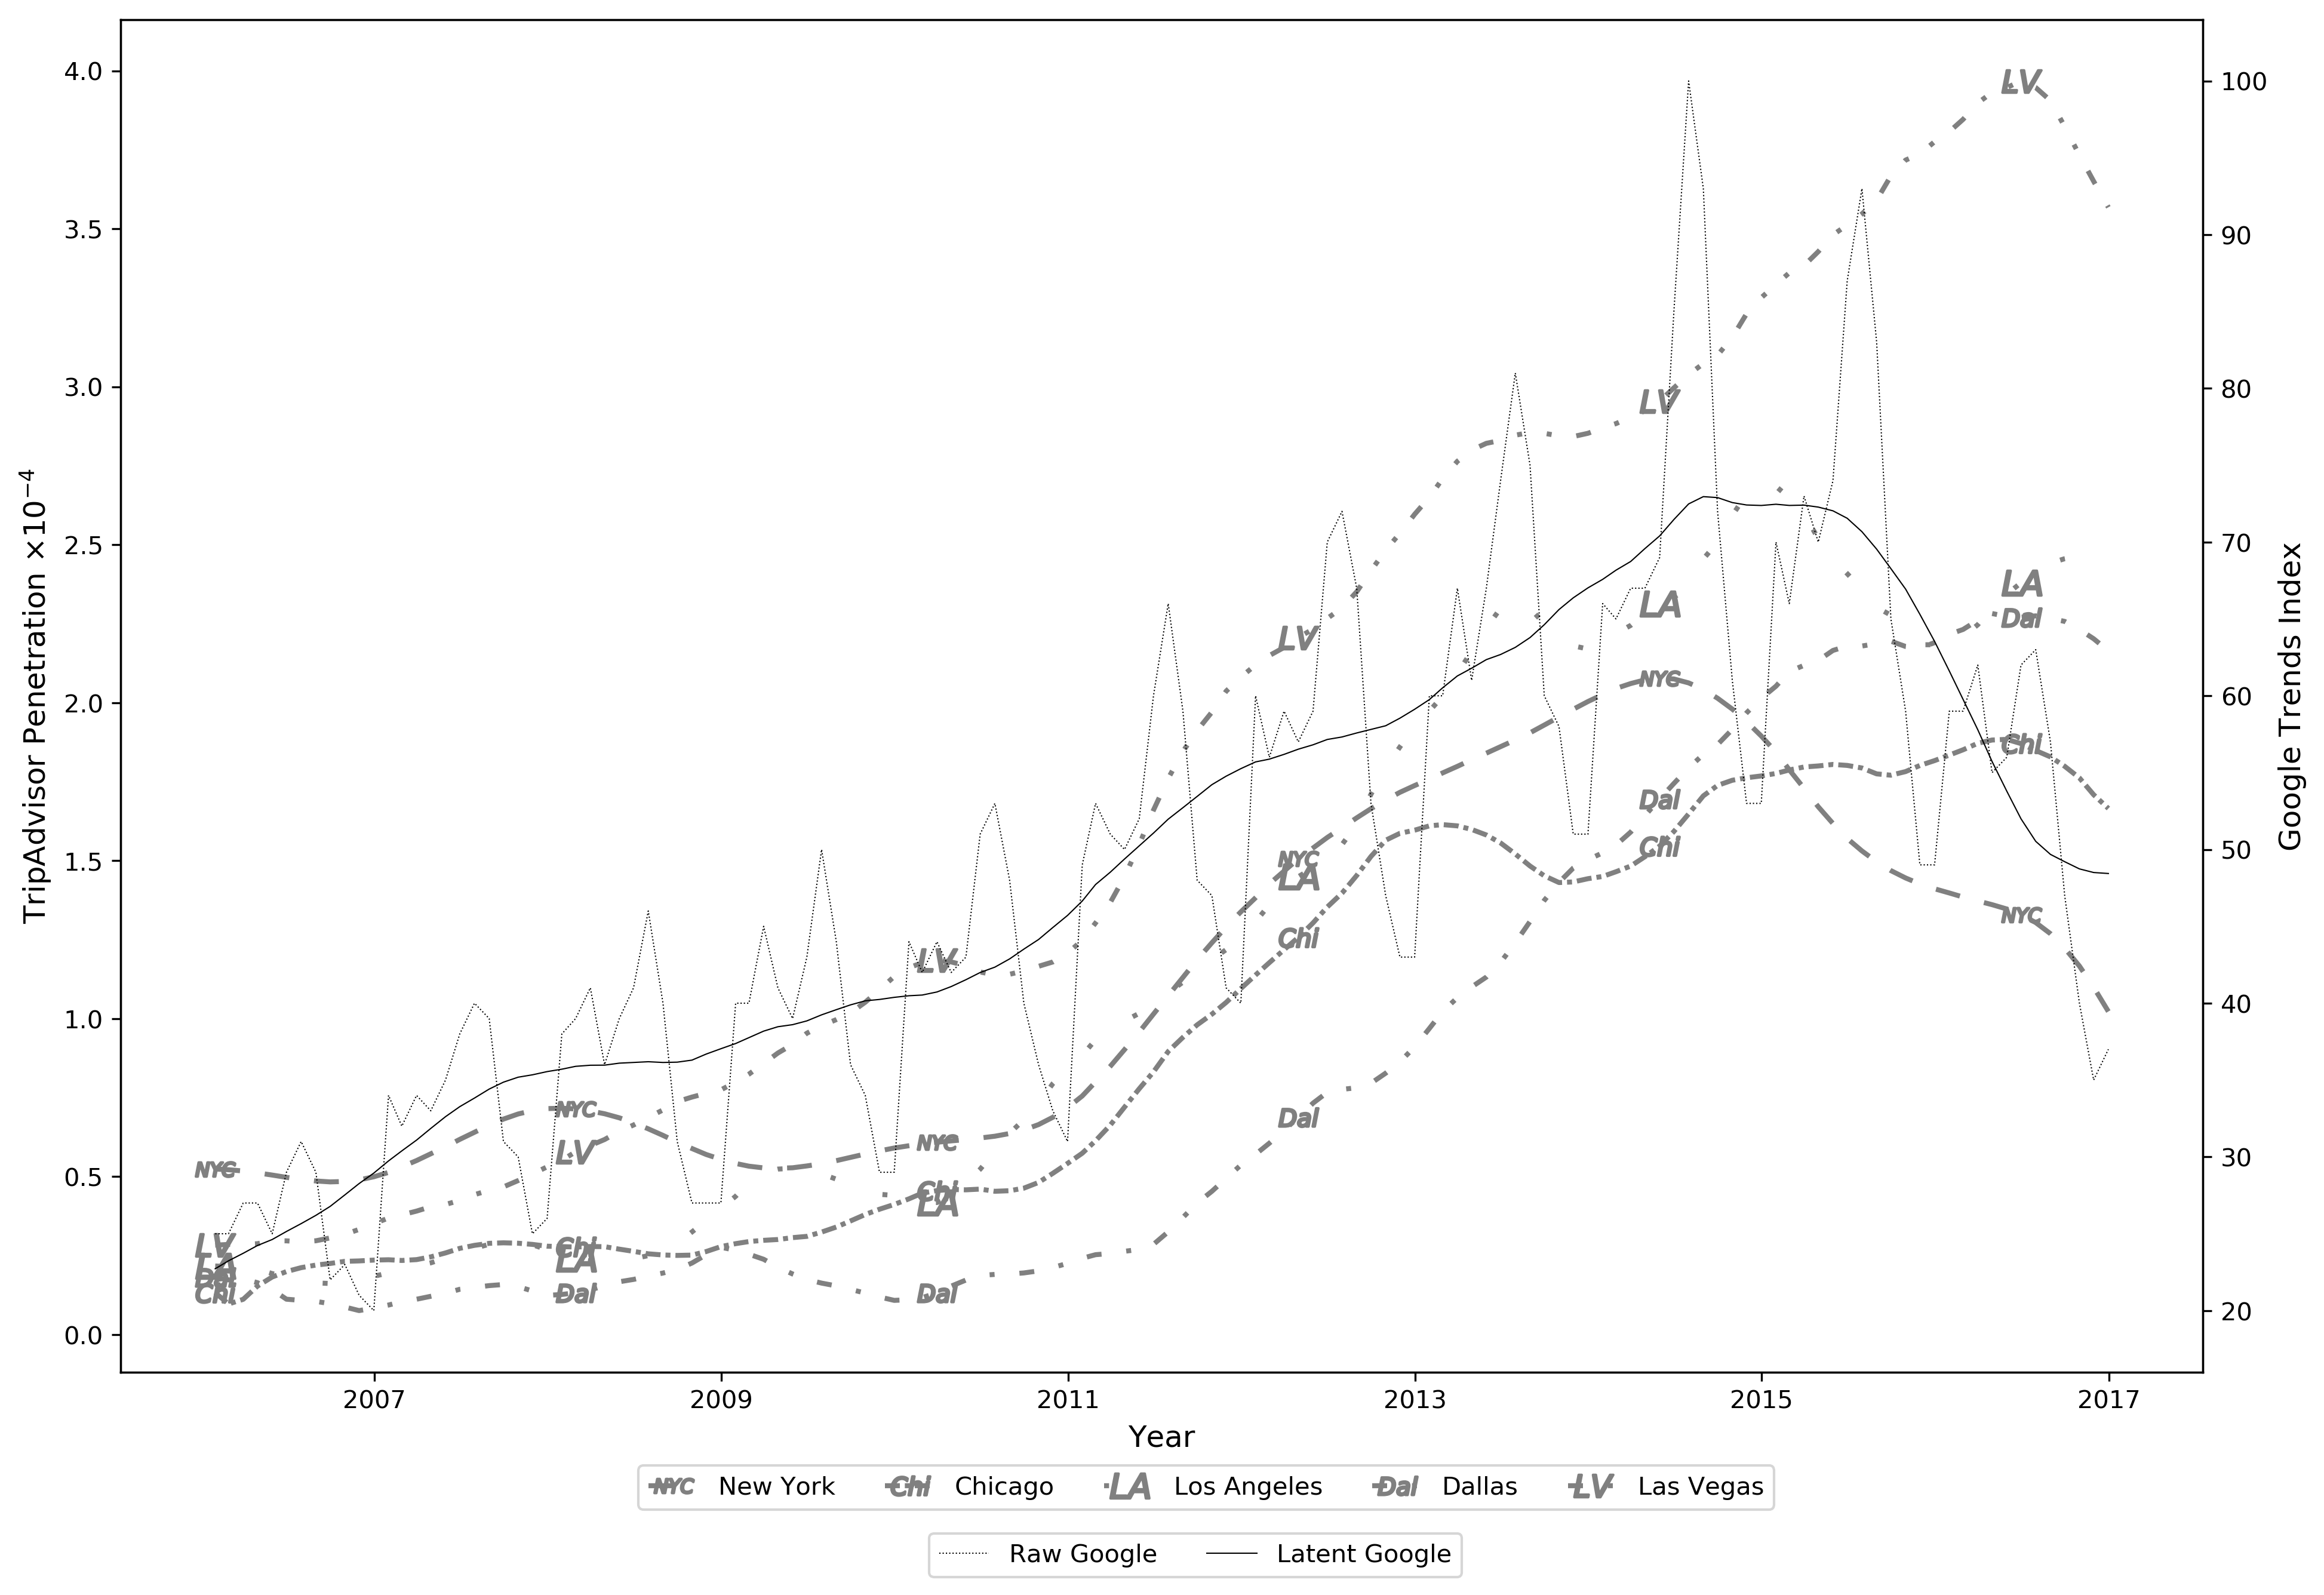
\includegraphics[width=0.8\textwidth,height=\textheight,keepaspectratio]{./Figures/TA_Penetration.png}}
{LATENT PENETRATION\label{fig:latentpen}}
{Shows TripAdvisor's Penetration (left y-axis) across major US cities over time. The rank order of market penetration changes; Dallas surpasses Chicago and New York. Google Trends Index (right y-axis) documents the Google search results for "TripAdvisor."}
\end{figure}
\clearpage

\begin{figure}[htp]
\FIGURE
{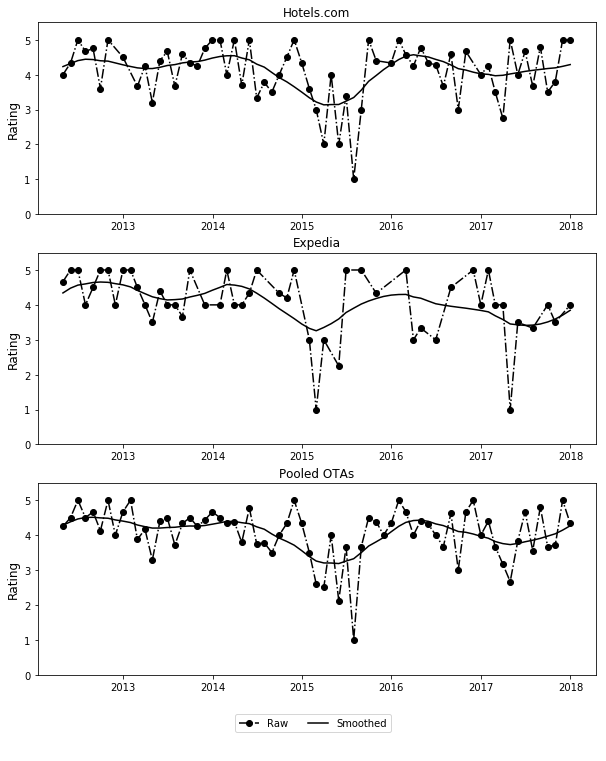
\includegraphics[width=0.8\textwidth,height=\textheight,keepaspectratio]{./Figures/Smoothed_Qual_18987_v2.png}}
{LATENT QUALITY: Embassy Suites (Memphis, TN) \label{fig:latentqual}}
{Comparing this hotel's raw ratings and latent quality as measured by  Hotels.com,  Expedia,  and  pooled  OTA  ratings.  The raw  ratings  are  noisy  while the latent quality trends are smooth.}
\end{figure}
\clearpage

\begin{figure}[htp]
\FIGURE
{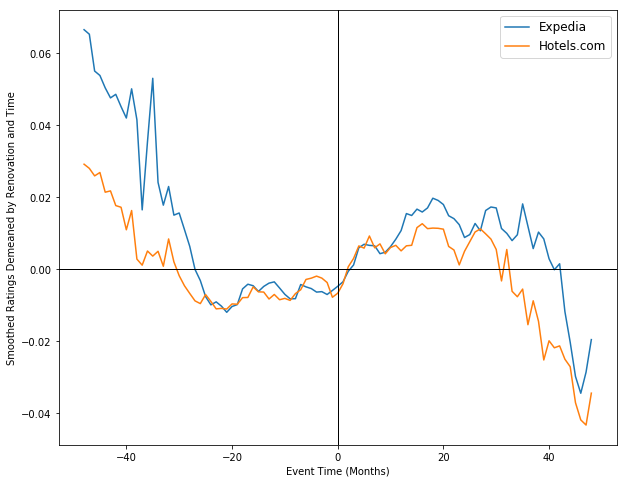
\includegraphics[width=0.8\textwidth,height=\textheight,keepaspectratio]{./Figures/Renovation_Event_dm_ym_event.png}}
{QUALITY CHANGES DURING RENOVATION EVENTS\label{fig:renovqual}}
{Demonstrates that, on average, hotels' quality is rapidly decreasing in the 5 years prior to the completion of a renovation and increases as the renovation progresses. The deterioration cycle seems to continue again around 3 years after the renovation.}
\end{figure}
\clearpage

\begin{figure}[htp]
\FIGURE
{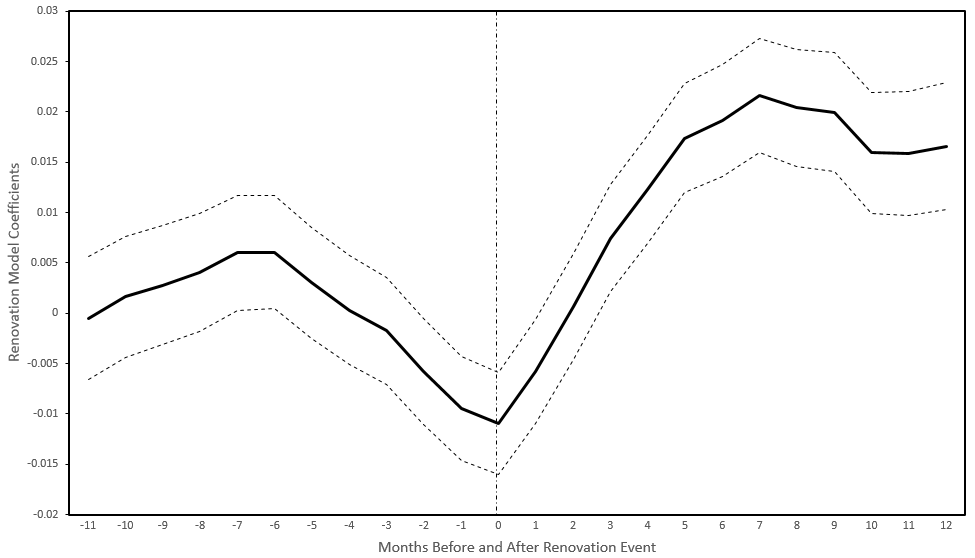
\includegraphics[width=0.8\textwidth,height=\textheight,keepaspectratio]{./Figures/Reno_Reg.png}}
{HOTEL RENOVATION\label{fig:reno_reg}}
{Demonstrates statistical evidence of hotel quality improvement due to renovation.}
\end{figure}
\clearpage

\begin{figure}[htp]
\FIGURE
{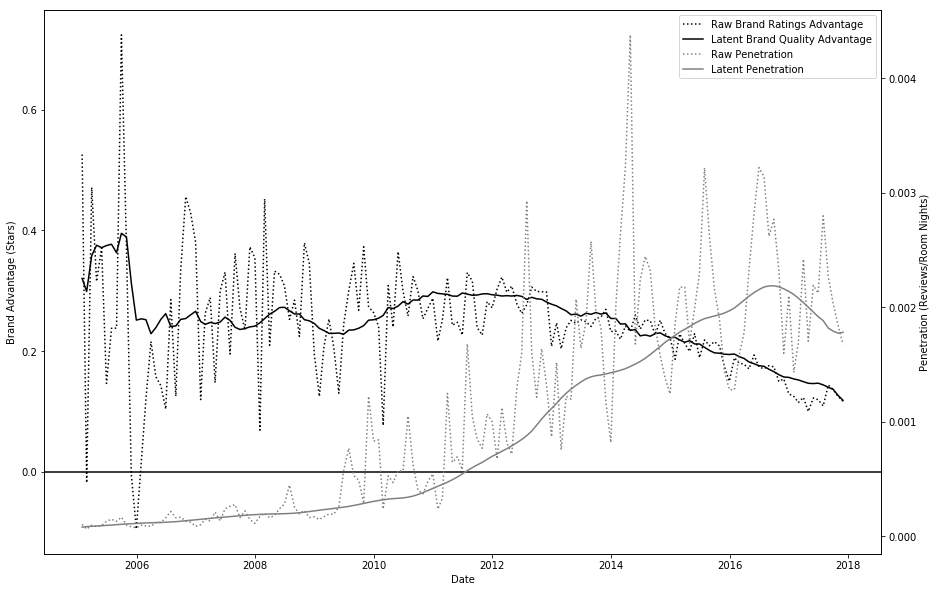
\includegraphics[width=0.8\textwidth,height=\textheight,keepaspectratio]{./Figures/OTA_Brand_v_Chain_v_PenetrationV2.png}}
{CHAIN ADVANTAGE BY TRIPADVISOR PENETRATION LEVEL\label{fig:modelfree}}
{Brand Quality Advantage (left y-axis) is the difference between the average quality of all chains' and average quality of all independents'. Average TripAdvisor penetration across all markets is plotted verses the right y-axis. Brand advantage decreasing as TripAdvisor penetration increases.}
\end{figure}
\clearpage

\begin{figure}[htp]
\FIGURE
{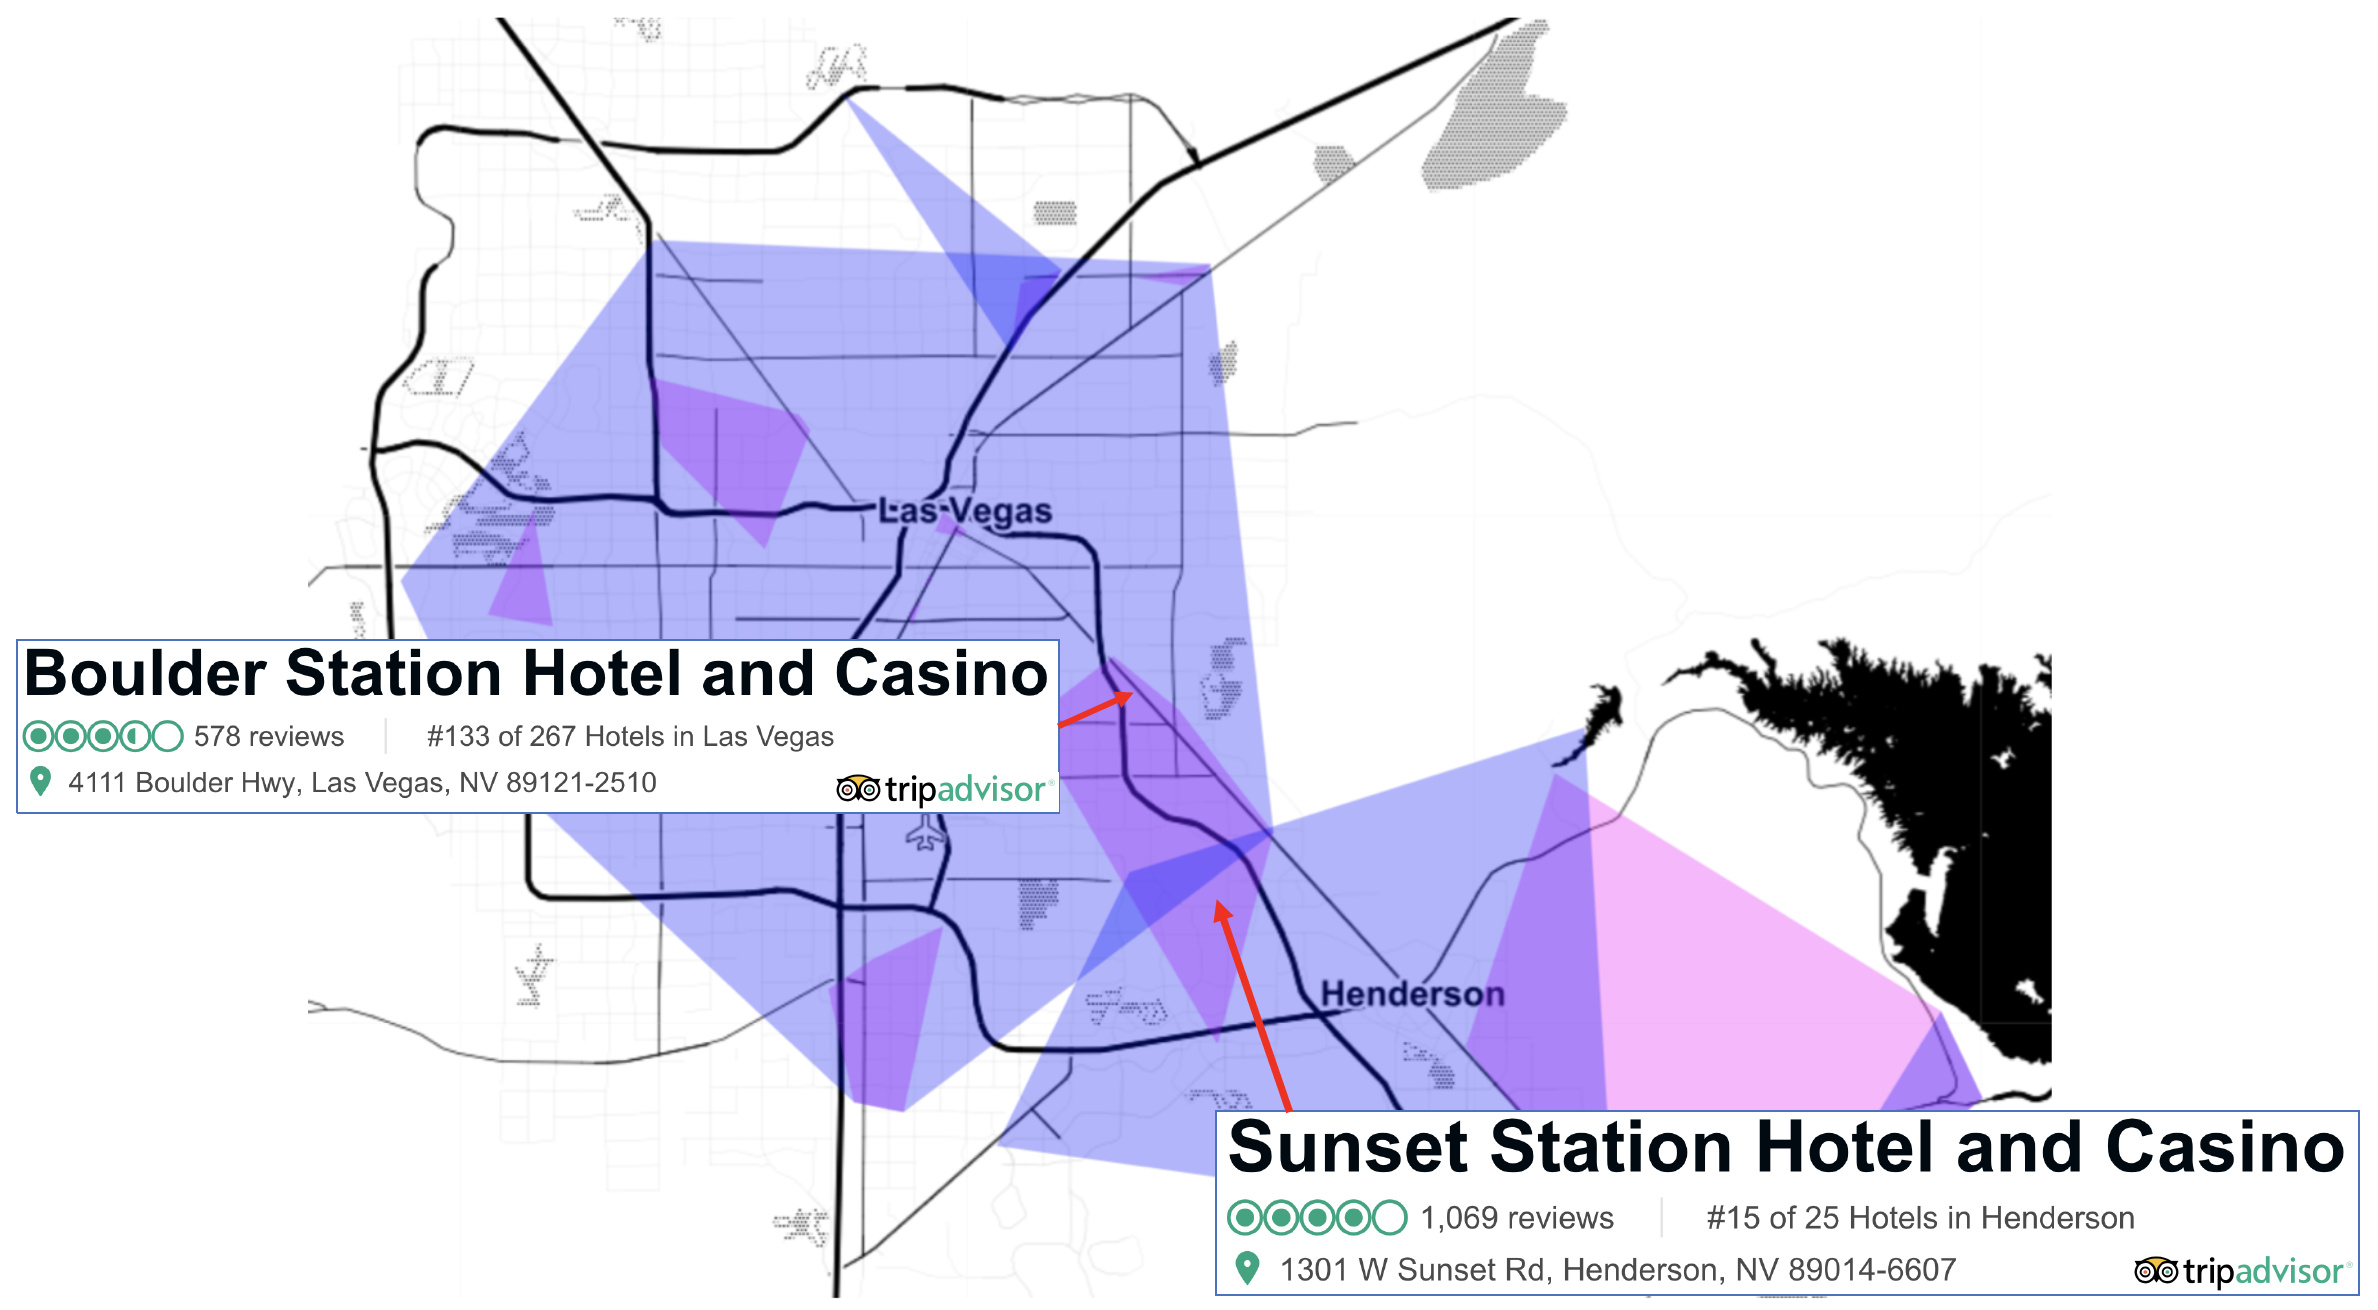
\includegraphics[width=0.8\textwidth,height=\textheight,keepaspectratio]{./Figures/LasVegasMarkets.png}}
{EXAMPLE OF LAS VEGAS MARKETS\label{fig:vegas}}
{Sam's Town and Skyline both belong to the Boulder Strip (as identified by HDBSCAN in pink) but belong to different TripAdvisor markets (as identified in blue). On TripAdvisor, they are ranked against hotels in their respective municipalities rather than against other hotels on the Boulder Strip.}
\end{figure}
\clearpage

\begin{figure}[htp]
\FIGURE
{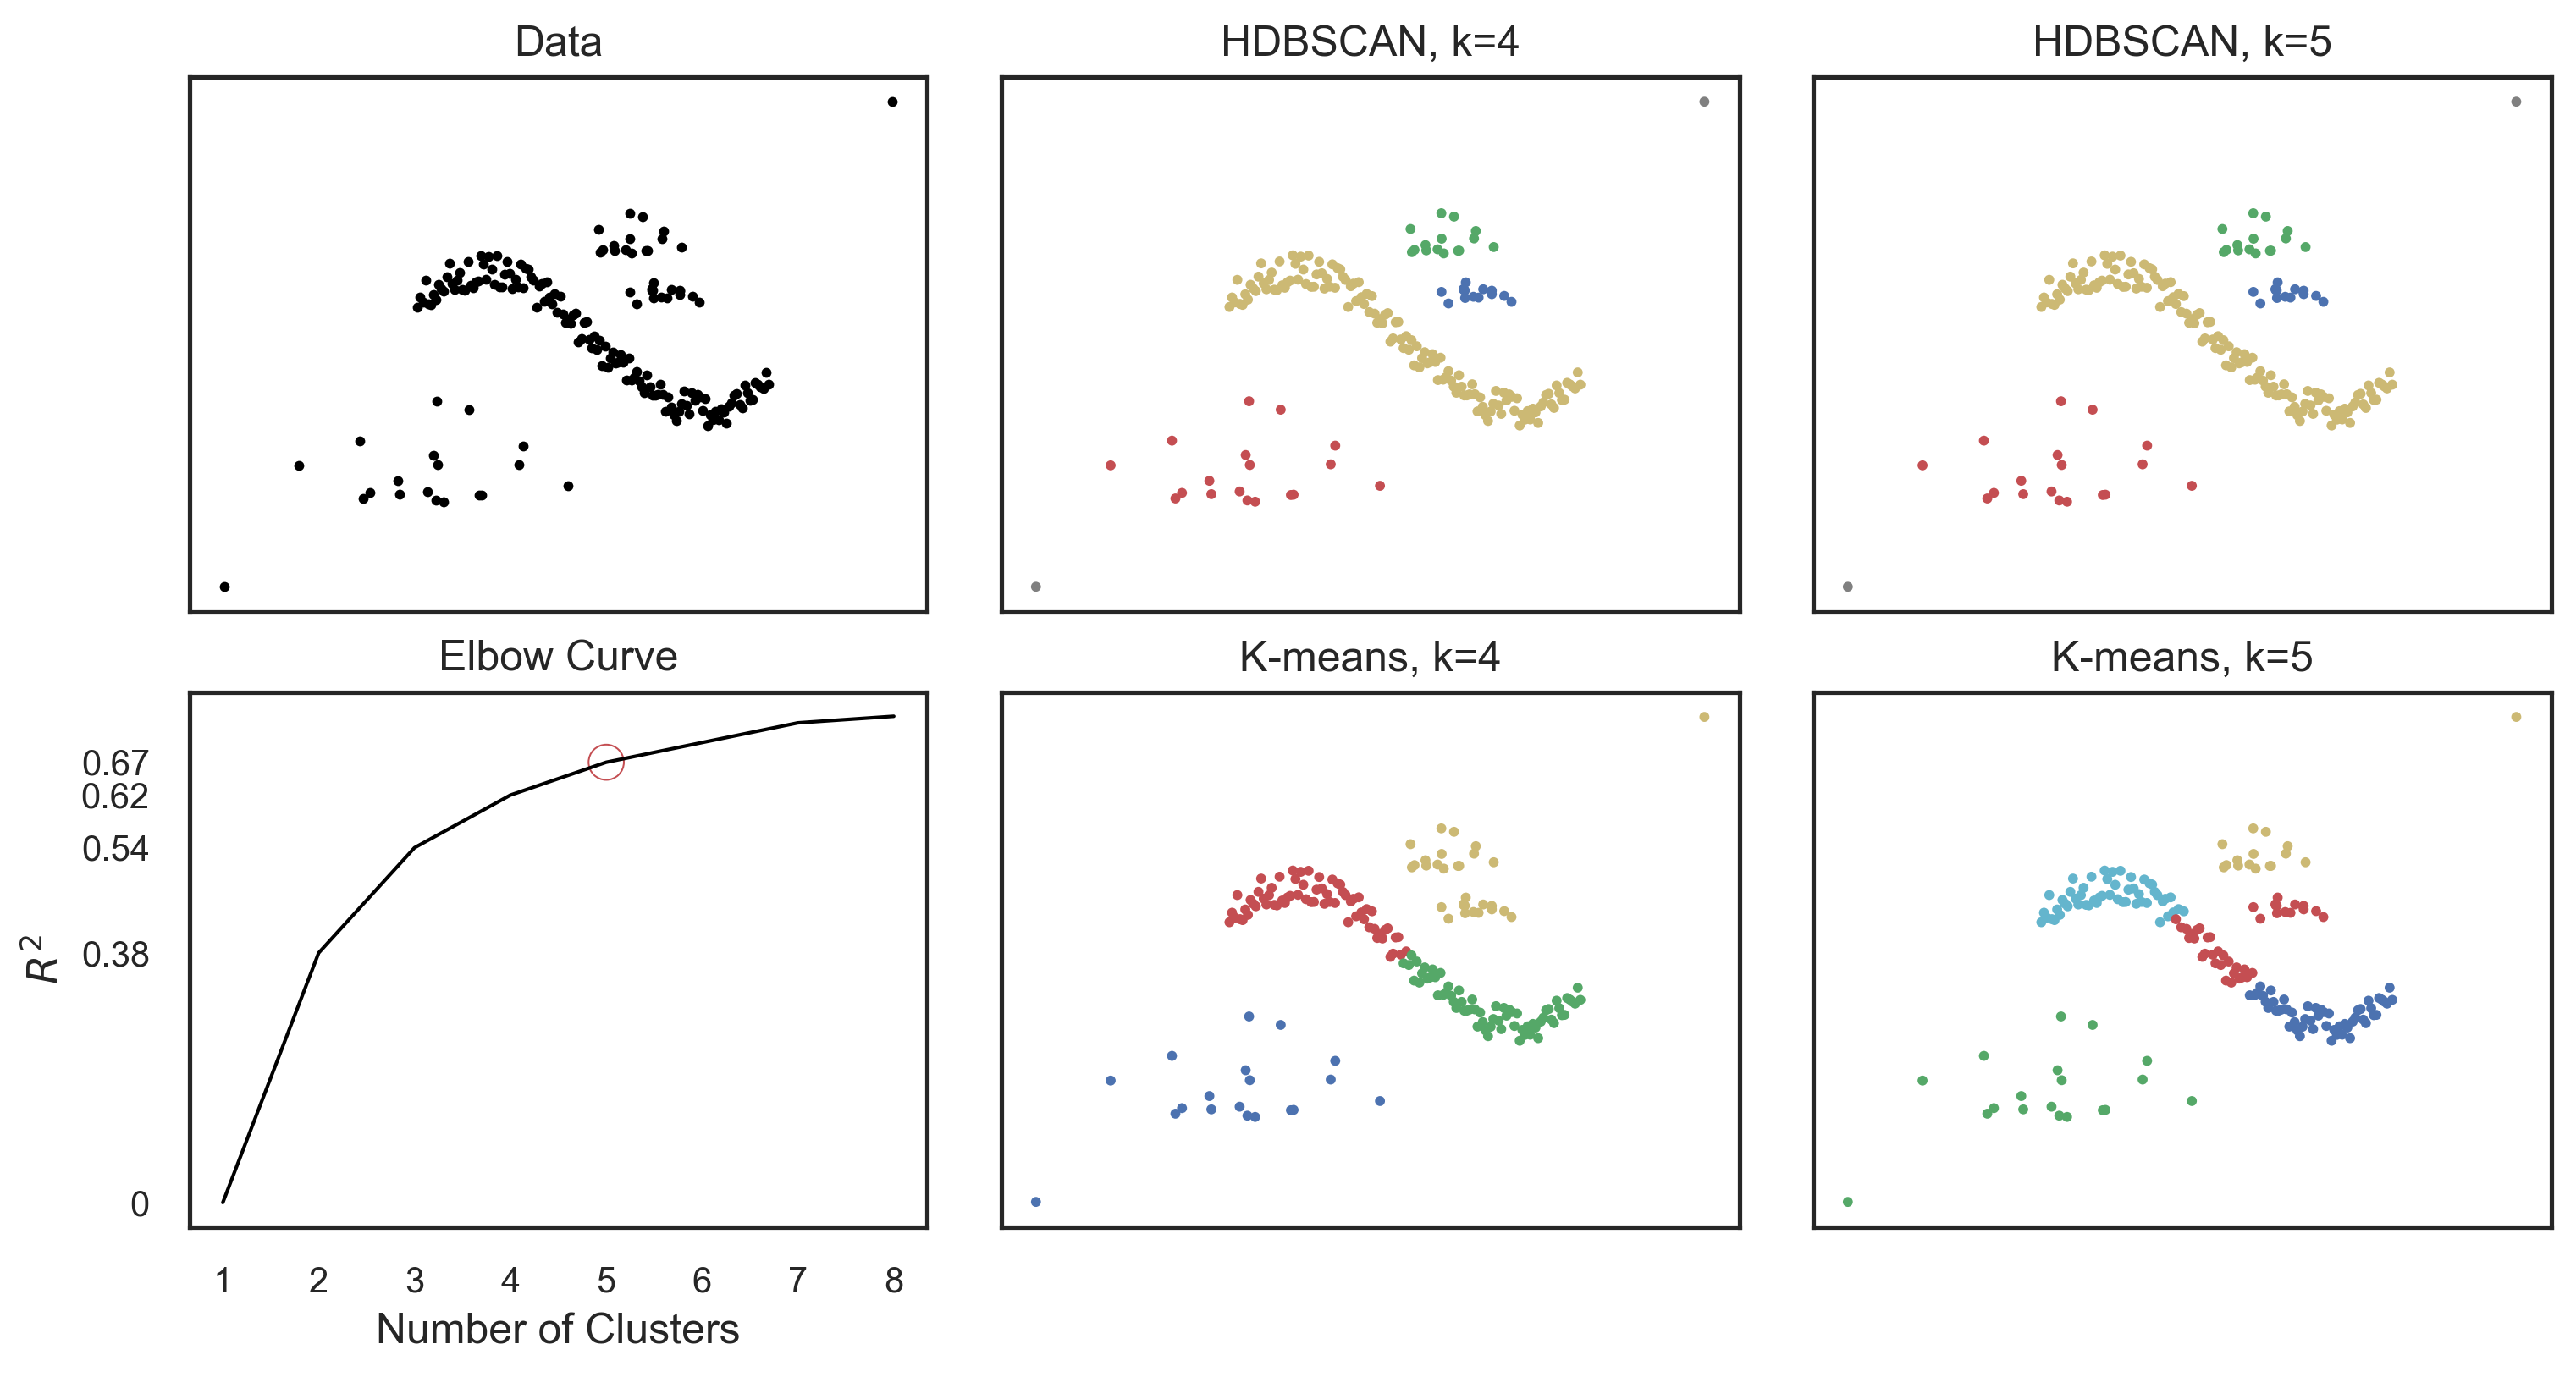
\includegraphics[width=0.8\textwidth,height=\textheight,keepaspectratio]{./Figures/clusters.png}}
{HDBSCAN AND K-MEANS COMPARISON\label{fig:cluster}}
{HDBSCAN is able to detect the visually intuitive clusters while k-means, a common clustering algorithm, struggles.}
\end{figure}
\clearpage


\begin{figure}[htp]
\FIGURE
{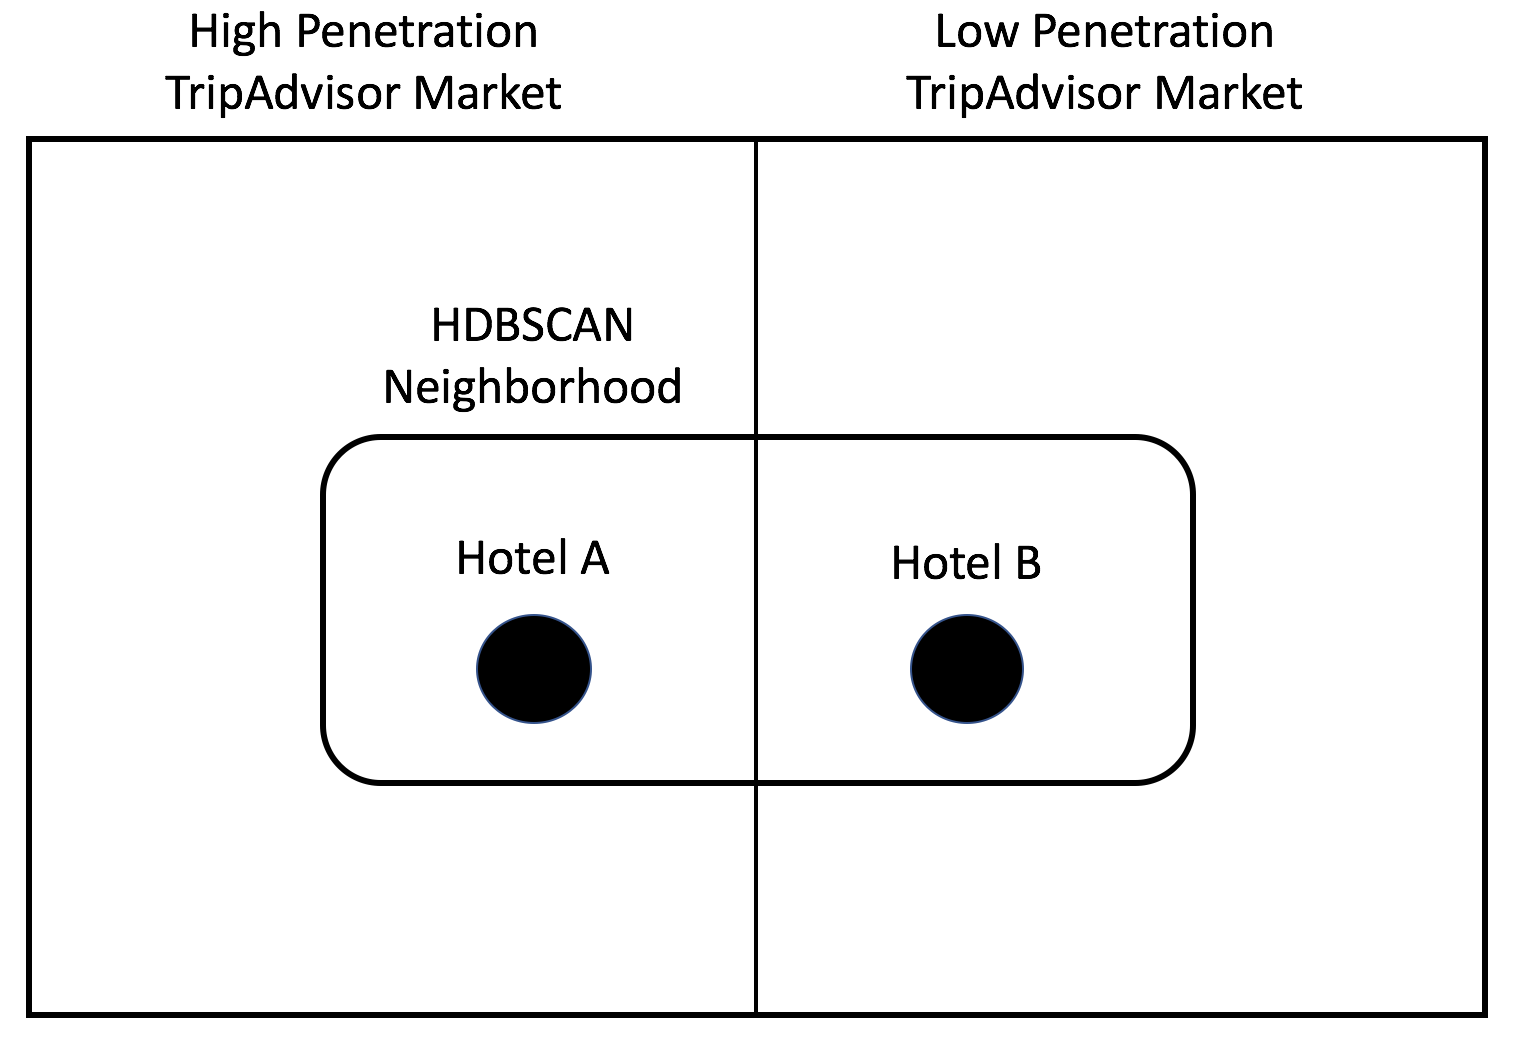
\includegraphics[width=0.8\textwidth,height=\textheight,keepaspectratio]{./Figures/Schematic.png}}
{SCHEMATIC REPRESENTATION OF EMPIRICAL TEST\label{fig:abmarkets}}
{}
\end{figure}
\clearpage

\begin{figure}[htp]
\FIGURE
{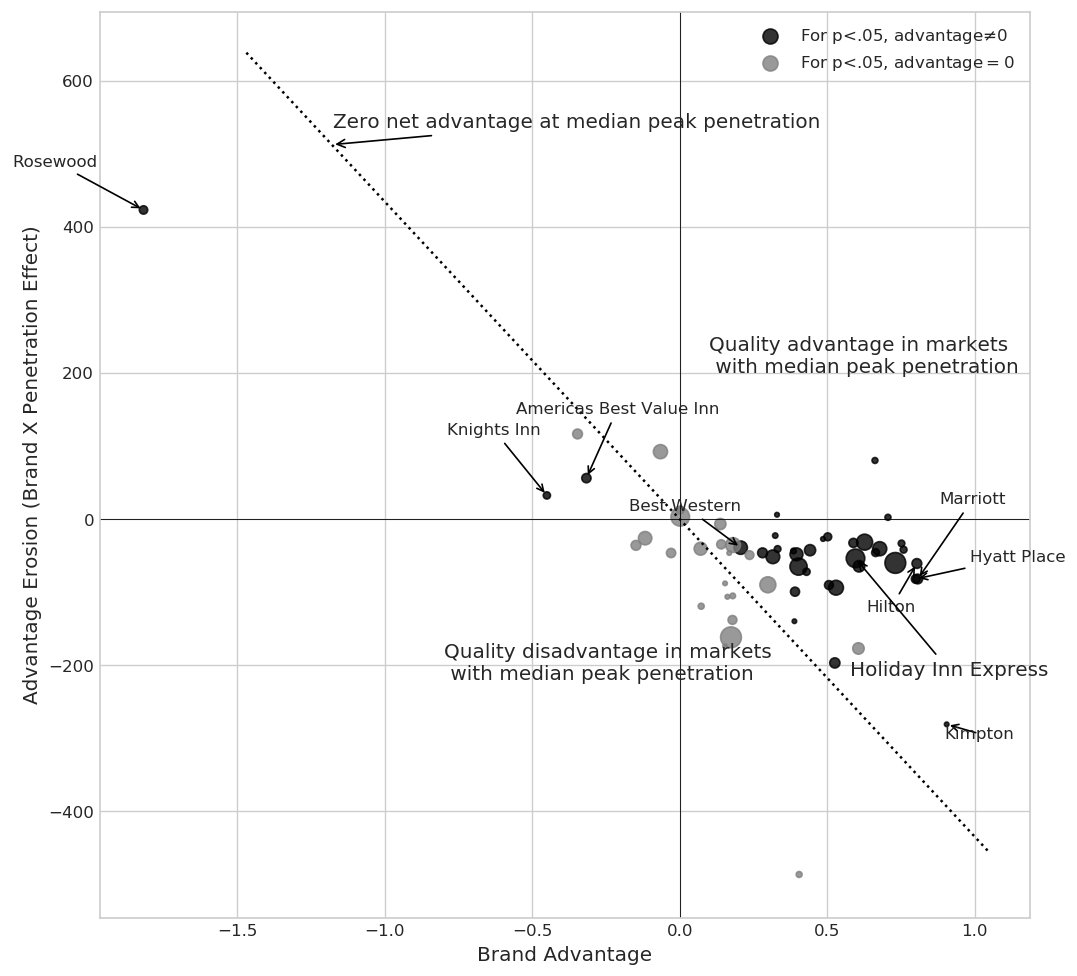
\includegraphics[width=0.8\textwidth,height=\textheight,keepaspectratio]{./Figures/brand_coeff2.png}}
{EROSION OF BRAND QUALITY ADVANTAGE\label{fig:brandvspenetrate}}
{This graph plots brand advantage (x-axis) versus the ddvantage erosion effect (brand$\times$penetration effect, y-axis), the black (gray) dots are brands with statistically significant (insignificant) quality advantages. The region above (below) the dotted diagonal line represents brands that hold a quality advantage (disadvantage) in a market with median levels of peak TripAdvisor penetration. The dots' diameters represent the relative total room capacities of brands.}
\end{figure}
\clearpage

% Acknowledgments here
\ACKNOWLEDGMENT{%
% Enter the text of acknowledgments here
}% Leave this (end of acknowledgment)


% Appendix here
% Options are (1) APPENDIX (with or without general title) or 
%             (2) APPENDICES (if it has more than one unrelated sections)
% Outcomment the appropriate case if necessary
%
% \begin{APPENDIX}{<Title of the Appendix>}
% \end{APPENDIX}
%
%   or 
%
% \begin{APPENDICES}
% \section{<Title of Section A>}
% \section{<Title of Section B>}
% etc
% \end{APPENDICES}

% References here (outcomment the appropriate case) 

% CASE 1: BiBTeX used to constantly update the references 
%   (while the paper is being written).
\bibliographystyle{informs2014} % outcomment this and next line in Case 1
\bibliography{references.bib} % if more than one, comma separated

% CASE 2: BiBTeX used to generate mypaper.bbl (to be further fine tuned)
%\input{mypaper.bbl} % outcomment this line in Case 2

\end{document}


